\documentclass{sig-alternate}

\usepackage{graphicx}
\usepackage{subfigure}
\graphicspath{.}

\usepackage{appendix}

% use this package if you need more space
\usepackage{times}

\usepackage{amsmath}
\usepackage{mathtools}
\usepackage{relsize}
\usepackage{verbatim}
\usepackage{color}
\usepackage{paralist}
\usepackage{tabularx}

%Theorem, Lemma, etc.
\usepackage[capitalise]{cleveref}
\newtheorem{theorem}{Theorem}
\newtheorem{definition}{Definition}
\newtheorem{lemma}{Lemma}
\newtheorem{proposition}{Proposition}
\newtheorem{corollary}{Corollary}
\newtheorem{example}{Example}

% Algorithms
\usepackage{algorithm}
\usepackage{algorithmic}
\renewcommand{\algorithmicrequire}{\textbf{Input:}}
\renewcommand{\algorithmicensure}{\textbf{Output:}}

% Floats
\usepackage{float}
\renewcommand{\textfraction}{0.00}
\renewcommand{\topfraction}{1.0}
\renewcommand{\bottomfraction}{1.0}
\setcounter{totalnumber}{100}
\setcounter{bottomnumber}{100}
\setcounter{topnumber}{100}

\newcommand{\TODO}[1]{{\bfseries\color{red}TODO: #1}}

\title{A Formal Treatment of the Task Assignment Problem in Spatial Crowdsourcing}
\begin{document}
%\numberofauthors{1}
%\author{{Mohammad Asghari, Liyue Fan, Cyrus Shahabi}\\
%\\
%\fontsize{10}{10}\selectfont\rmfamily\itshape
%Integrated Media Systems Center, University of Southern California\\
%\fontsize{9}{9}\selectfont\ttfamily\upshape
%\{masghari, liyuefan, shahabi\}@usc.edu\\
%}

\maketitle
\begin{abstract}
Abstract
\end{abstract}

\section{Introduction}

Smartphones are ubiquitous: we are witnessing an astonishing growth in mobile phone subscription. The International Telecommunication Union estimates there are nearly 7 billion mobile subscriptions world wide \cite{Mobiforge14}. Meanwhile, the mobile phone’s bandwidth is constantly increasing: from 2.5G (up to 384Kbps) to 3G (up to 14.7Mbps) and recently 4G (up to 100 Mbps) (Sauter, 2011). Hence, the multiplication of the above two factors plus the constant progress and increase of smartphone’s sensors (e.g., video cameras) suggest an exponential growth in data collection and sharing by smart phones. That is, every person with a mobile phone can now act as a multi-modal sensor collecting and sharing various types of high-fidelity spatiotemporal data instantaneously (e.g., picture, video, audio, location, time, speed, direction, and acceleration).

Exploiting this large volume of potential users and their movability, a new mechanism for efficient and scalable data collection has emerged: \emph{Spatial Crowdsourcing}\cite{Kazemi12}. Spatial crowdsourcing requires workers (e.g., willing individuals) to perform a set of tasks by physically traveling to certain locations at particular times. Spatial crowdsourcing has applications in numerous domains such as journalism, tourism, intelligence, disaster response and urban planning. With spatial crowdsourcing, the requester issues a query to a spatial crowdsourcing server (SC-Server). Consequently, the SC-server distributes the query among the available workers in the vicinity of the events. Once the workers document their events with their mobile phones, the results are sent back to the requester.

The main challenges of spatial crowdsourcing are due to the large-scale, ad-hoc and dynamic nature of the workers and tasks.  First, to continuously match thousands of spatial crowdsourcing campaigns, where each campaign consists of many spatiotemporal tasks, with millions of workers, an SC-Server must be able to run efficient task-assignment strategies that can scale.  Second, the task-assignment must be performed frequently and in real-time as new tasks and workers become available or as tasks are completed (or expired) and workers leave the system. Finally, individuals with mobile devices need to physically travel to the specified locations of interest. An adversary with access to individual whereabouts can infer sensitive details about a person (e.g., health status and political views); thus, protecting worker location privacy is an important concern in spatial crowdsourcing.




\section{Preliminaries}
\label{sec:prelim}

In this section, we define the terminologies used in the paper and give a formal definition of the problem under consideration. In addition, we analyze the complexity of the problem and its hardness.

\subsection{Problem Definition}
\label{subsec:problemdef}

We start by defining some terminologies in order to formally define the task assignment problem in spatial crowdsourcing.

\begin{definition} [Spatial Task]
A spatial task t is a task to be performed at location t.l with geographical coordinates, i.e., latitude and longitude. The task becomes available at t.r (release time) and expires at t.d (deadline). Also, t.v is the obtained reward after completing t.
\end{definition}

It should be pointed out that in a spatial crowdsourcing environment, a spatial task \emph{t} can be executed only if a worker is at location \emph{t.l}. For example, if the query is to report the traffic situation at a specific location, someone has to actually be present at the location to be able to report the traffic. From here on, whenever we use \emph{task} we are actually referring to a spatial task. Now, we formally define a worker.

\begin{definition} [Worker]
A worker w is any entity, e.g., a person, willing to perform spatial tasks. We show the current location of the worker by w.l. Each worker has a list of tasks assigned to it, w.T, and a maximum number of tasks it is willing to perform, w.max. Also w.s and w.e show the availability of the worker such that the worker is available during the time interval $\left( w.s, w.e \right]$.
\end{definition}

Throughout the paper we assume every worker moves one unit of length per unit of time. Therefore, we can assume that $distance \left( \left\langle a,b \right\rangle \right)$ is also the \emph{time} required to move from point $a$ to point $b$.

\begin{definition} [Schedule]
We call an ordered list of tasks a schedule. We show s as $\left\langle t_1, ..., t_n \right\rangle$ where n is the number of tasks in s. If we show the $i^{th}$ task in s with $s_i$, we say worker w is able to perform schedule s if and only if:
\begin{equation*}
\forall i, 1\leq i \leq n \ \ \ \ \sum_{j=1}^i distance(s_{j-1}, s_j) \leq s_i.d
\end{equation*}
where $s_0.l$ is the current location of the w.
\end{definition}

At each point in time, each worker keeps track of a schedule and completes the tasks based on their order in its schedule.

\begin{definition} [Matching]
Assuming we have a set of workers W and a set of tasks T, we call $M \subset W \times T$ a matching if for each $t \in T$ there is at most one $w \in W$ such that $\left( w, t \right) \in M$. We call $\left( w, t \right) \in M$ a \emph{match} and say t has been matched to w. For each matching M, we define the value (benefit) of M as:
\begin{equation*}
Value(M) = \sum_{\left( w, t \right) \in M} t.v
\end{equation*}
\end{definition}

\noindent A matching $M$ is valid if and only if, for every worker $w$, there exists a schedule $s$, such that $(w, t_i) \in M \implies t_i \in s$. 

Now we can formally define the Task Assignment in Spatial Crowdsourcing (TASC) as follows:

\begin{definition}[Task Assignment in SC]
Given a set of workers $W$, a set of spatial tasks $T$ and a cost function $d: \left( W \cup T \right) \times T \rightarrow \mathbb{R}$ where $d \left( \left\langle a,b \right\rangle \right)$ is the distance between $a$ and $b$, the goal of the TASC$\left\langle W, T, d \right\rangle$ problem is to find a valid matching $M$ with maximum value.
\end{definition}

It is important to note that with task assignment in SC, the goal is to find a \textit{valid matching}. This means that in addition to finding a \textit{matching} between tasks and workers, SC-Server has to also find a \textit{schedule} for each worker to perform the tasks. Throughout this paper we use the terms \textit{matching phase} and \textit{scheduling phase} to refer to the two different aspects of task assignment in SC. We focus on maximizing the total number of assignment and hence we assume every task has a value equal to 1. \cref{tab:notation} lists the notations we frequently use in this paper.\\

\begin{table}
\begin{center}
\begin{tabular}{| c | l |} \hline
Notation	&	Description \\ \hline
$t.l$			&	location of task $t$ \\ \hline
$t.r$			&	release time of task $t$ \\ \hline
$t.d$		& 	deadline of task $t$ \\ \hline
$t.v$		&	value of task $t$ \\ \hline
$w.l$		&	location of worker $w$ \\ \hline
$w.s$		&	the time worker $w$ becomes available \\ \hline
$w.e$		&	the time worker $w$ becomes unavailable \\ \hline
$w.T$		&	list of tasks assigned to worker $w$ \\ \hline
$w.max$	&	maximum number of tasks worker $w$ \\
				&	performs \\ \hline
$w.PTS$	&	list of all potential task subsets worker $w$ \\
				&	can perform \\ \hline
\end{tabular}
\caption{List of notations}
\label{tab:notation}
\end{center}
\end{table}

\subsection{Complexity Analysis}

The equivalent decision problem for TASC is to decide if there exists a matching $M$ with value $K$ and is denoted as TASC$\left\langle W, T, l, K \right\rangle$. In this section we use a slightly modified version of the well known Hamiltonian Path Problem. We call it the Minimum Length Hamiltonian Path Problem (Min-Ham-Path) and define it as follows:

\begin{definition}[Min-Ham-Path]
Given a directed graph $G(V,E)$ where each edge $e \in E$ is assigned a length $l: E \rightarrow \mathbb{R}$, a source node $s$ and a length $L \in \mathbb{R}$, the Min-Ham-Path problem $\left\langle G, l, s, L \right\rangle$ is to decide whether there exists a path in $G$ that starts from $s$, visits every other node exactly once and has a length of at most $L$.
\end{definition}

\begin{theorem}
\label{th:MinHam}
The Min-Ham-Path problem is NP-Hard.
\end{theorem}

\begin{proof}
%Proof is shown in \cref{app:MinHamProof}.
In order to prove NP-Hardness of Min-Ham-Path we show Ham-Path $\leq_p$ Min-Ham-Path. The Hamiltonian Path problem asks the following question: Given a directed graph $G(V,E)$ does there exist a path that goes through every node exactly once?

Given and instance of the Ham-Path problem $\left\langle G \right\rangle$ we modify graph $G(V,E)$ and generate a new graph $G'(V', E')$ where $V' = V \cup \left\{ o \right\}$ and $E' = E \cup \left\{ \left\langle o, v \right\rangle : v \in V \right\}$. Also, for every $e \in E'$ we Assume $l(e) = 1$.

Now we show that Ham-Path$\left\langle G \right\rangle$ is true if and only if Min-Ham-Path$\left\langle G', l, o, n \right\rangle$ is true where $n$ is the number of vertices in $G$. If Min-Ham-Path returns a path of length $n$, we can remove the first edge from the path which results in a Hamiltonian Path for the Ham-Path$\left\langle G \right\rangle$ problem. On the other hand every Hamiltonian Path on graph $G$ has length $n-1$. By adding vertex $o$ and connecting it to the starting vertex, we end up with a Hamiltonian Path of length $n$ on $G'$.
\end{proof}

\begin{theorem}
\label{th:TASC}
The TASC problem is NP-Complete.
\end{theorem}

\begin{proof}
%Proof is shown in \cref{app:TASCProof}
We start the proof by showing that the decision problem of TASC is \textit{verifiable} in polynomial time. Given a matching $M$, we can check that no task is assigned to more than one worker in polynomial time. Furthermore, based on the definition of a valid match, checking the validity of a matching $M$ in polynomial time. Finally, we can find the value of $M$ by adding the value of every task in $M$.

We show TASC is NP-Hard by proving the reduction Min-Ham-Path $\leq_p$ TASC. Given an instance of the Min-Ham-Path problem $\left\langle G(V,E), l, o, K \right\rangle$ we reduce it to an instance of the TASC$\left\langle W, T, l', n-1 \right\rangle$ problem such that $W = \left\{ o \right\}$, $T = V \setminus \left\{ o \right\}$. For every task $t$ we set $t.v = 1$, $t.r = 0$ and $t.d = K$. Also for every $e \in E, l'(e) = l(e)$. In addition for every $e' \in \left( W \times T \right) \cup \left( T \times T \right) $ where $e' \not\in E$ we set $l'(e') = \infty$.

Finally we show the result of Min-Ham-Path$\left\langle G, l, o, K \right\rangle$ is true if TASC$\left\langle W, T, l', n-1 \right\rangle$ is true where $n$ is the number of vertices in $G$. Considering that $\left\vert T \right\vert = n - 1$ and $t.v = 1$ for every $t \in T$, if there exists a matching with size $n - 1$ it means every task has been assigned to the single worker. Also, since the deadline of every task is $K$ the worker visits every task no later than $K$. Therefore, the path that the worker traverses starts at $o$ and goes through every other vertex $v \in V \setminus \left\{ o \right\}$, where the length of the path is no more than $K$.
\end{proof}

\vspace{-0.05in}
\section{Related Work}
\label{sec:related}
\vspace{-0.1in}
Many studies in spatial crowdsorcing research focus on the task assignment problem\cite{Kazemi12,Deng13,Li15,Chen15,Deng15,Cheng16,Fonteles15,Guo16}. Kazemi and Shahabi\cite{Kazemi12}, Cheng et. al.\cite{Cheng16} and Fonteles et. al.\cite{Fonteles15} formulate task assignment in spatial crowdsourcing as a matching problem. In \cite{Kazemi12,Fonteles15} the primary objective is to maximize the number of matched tasks while in \cite{Cheng16} the minimize the distance between the tasks and their matched workers. Furthermore, neither of these studies consider the schedule of a worker when matching tasks and workers. Deng el. al.\cite{Deng13} and Li et. al\cite{Li15} study the problem of scheduling tasks that have already been asigned to a worker. While in \cite{Deng13} all matched tasks are available at the time scheduling is performed, the authors look at the online version of the same problem in \cite{Li15} where the scheduling algorithm is performed immediately after a new task gets matched with the worker. More recent studies have considered both matching and scheduling using the batched scheme \cite{Chen15,Deng15,Guo16}. Chen et. al.\cite{Chen15} formulate the problem as in Integer Linear Program where the objective is to minimize the total traveled distance of the workers. In \cite{Deng15}, to process each batch, the algorithm first performs matching and then tries to schedule the matched tasks. For those tasks that did not get scheduled another round of matching and scheduling is performed and this continues until either all tasks are scheduled or there is no eligible worker remained for an unscheduled task. In \cite{Guo16}, Guo et. al. propose greedy-enhanced genetic algorithms for matching and scheduling time-sensitive and time-insensitive tasks separately. 

Our work is also related to some combinatorial optimization problems such as Vehicle Routing Problem(VRP) \cite{Braysy05}. The general setting of VRP is to serve a number of customers with a fleet of vehicles and the objective is to minimize the total travel cost of those vehicles. Compared with VRP, with spatial crowdsourcing our objective is to maximize the number of completed tasks, whereas VRP aims to minimize the total travel time. In addition, the spatial workers in our problem setting are not located at one or several fixed depots, and each worker can show up at any unique location. In our setting the spatial tasks are also not guaranteed to be completed by the workers. 
%Finally, in a spatial crowdsourcing platform, we need to provide efficient solutions for potentially millions of tasks and workers. This is different from the solutions in VRP which take hundreds of seconds even for one hundred delivery points.

%Auction frameworks have been used in various domains such as dynamic multi-agent environments \cite{Mehta05,Lagoudakis04} and online advertising \cite{Ghosh10}. Bidding strategies from other domains cannot be used in spatial crowdsourcing as they do not consider the spatial and temporal characteristics of SC. In this paper, we develop bidding strategies that are unique to a spatial crowdsourcing environment. One aspect of auction frameworks that has been widely studied is how to prevent bidders from submitting malicious bids to give themselves unfair advantage \cite{Lavi05}. This problem does not apply to our Auction-SC framework because here, the workers do not directly interact with the SC-Server. Instead, the software on a worker's phone receives tasks, computes bids and submits them to the server. If a task is assigned to a worker, the worker will be notified with an updated schedule through the software. The worker has no control over the software and hence, cannot cheat the system.

%Some recent studies in spatial matching \cite{Wong07,Long13} do focus on efficiency and use the spatial features of the objects for more efficient assignment. These studies assume a global knowledge about the locations of all objects exists a priori and the challenge comes from the complexity of spatial matching. However, spatial crowdsourcing differs due to the dynamism of tasks and workers (i.e., tasks and workers come and go without our knowledge), thus the challenge is to perform the task assignment at a given instance of time with the goal of global optimization across all times. Moreover, the fact that workers need to travel to task locations causes the landscape of the problem to change constantly. This will add another layer of dynamism to spatial crowdsourcing that makes it a unique problem.

%One can consider the task assignment problem in spatial crowdsourcing as a matching problem between tasks and workers, which makes it similar to the classic matching problem \cite{Gibbons85,Avis83}. In particular, the online matching problem \cite{Kalyanasundaram93, Kalyanasundaram00} is the most relevant variation to spatial crowdsourcing as it captures the dynamism of tasks arriving at different times. However, once the number of tasks assigned to one worker is more than one, the online matching problem cannot capture the true cost of performing tasks. More specifically, once you assign a set of tasks to a worker, the cost of executing this set is the distance of the shortest path that starts from the worker’s current location and goes through the locations of all the assigned tasks. On the other hand, with online b-matching \cite{Kalyanasundaram00} the overall cost for one worker would be the sum of the distances between the worker and each assignedtask.

%Modeling the assignment cost as the shortest path a worker has to take to visit the locations of multiple tasks, brings another class of problems to attention. In this context the assignment problem in spatial crowdsourcing becomes similar to the Traveling Salesman Problem (TSP) \cite{Lawler85} and the Vehicle Routing Problem (VRP) \cite{Toth02}. The online versions of both TSP and VRP have been studied to some extent where new locations to visit are revealed incrementally. Since there is only one salesman in the standard version of TSP, here we focus on VRP. Different variations of VRP have been studied, yet there are still some differences between task assignment in spatial crowdsourcing and these variations. In VRP, a server can pay a penalty and deny visiting a location; however, in spatial crowdsourcing the goal is to maximize the number of assigned tasks so the worker does not have the option of denying a task. Furthermore, in VRP, all servers start from the same depot where in spatial crowdsourcing each worker can have a different starting location. Moreover, in VRP we have a fixed number of servers whereas in spatial crowdsourcing the same type of dynamism for tasks can apply to the workers. That is, workers can be added (removed) to (from) the system at any time.


\section{Exact Clairvoyant Algorithm}
\label{sec:exactalgo}

% In a real world crowdsourcing environment, the server has no information with regard to tasks (workers) becoming available in the future. The server becomes aware of a task (worker) and all its subsequent information only when the task (worker) becomes available. Due to this lack of knowledge, at each time, the server might make an assignment that will prove not to be towards an optimal solution once more information becomes available in the future. 

%In order to solve the TASC problem, the server requires a global knowledge of all the current and incoming spatial tasks and workers. In such case, the server can assign tasks to workers such that the value of the matching is maximized. However, the server does not have such global knowledge. The server will become aware of a task (worker) and all its corresponding information once the task (worker) becomes available. Due to this lack of future knowledge, finding a globally optimal solution is not feasible.\\

In order to have a benchmark to evaluate our real-time algorithms, in this section, we define a clairvoyant off-line algorithm. We assume there exists a clairvoyant which has a global knowledge of tasks and workers. In this case, the clairvoyant can assign tasks to workers such that the value of the matching is maximized. We propose a two step algorithm which finds the optimal solution to TASC problem. In the first step we find all potential subsets of tasks that a single worker is able to complete. Having the output of step 1, in the next step we find a matching with maximum value. In the following, we describe different steps of the algorithm and later discuss the complexity of the algorithm. We also show how to adapt the algorithm to address a more general spatial crowdsourcing framework. This adaption does not deteriorate the performance of the algorithm, and in most cases even improves it.

\subsection{Discovering Potential Task Subsets}
\label{subsec:FindPTS}
In the first step of the algorithm we focus on finding all task subsets that a worker \emph{w} is be able to complete. We can define a Potential Task Subset as:

\begin{definition} [Potential Task Subset]
\label{def:PTS}
We call $PTS \subset T$ a potential task subset for worker w iff there exists a route that starts from w.l and for every $t \in PTS$ the path visits t.l at time $\delta$ such that $t.r \leq \delta < t.d$. Also the path should not start earlier than w.s and end before w.e. We define the value of PTS as:
\begin{equation*}
Value(PTS) = \sum_{t \in PTS} t.v
\end{equation*}
\end{definition}

For each worker \emph{w}, we define \emph{w.PTS} as the set of all such potential task subsets.

In order to find all PTSs for a single worker, a straightforward method is to go through all subsets of \emph{T} and check whether it is a PTS for the worker or not. It is trivial to see that such approach requires $O(n!)$ permutations which makes it computationally expensive. Therefore, we utilize a branch and bound algorithm similar to the one introduced in \cite{Deng13}. We use the following propositions for pruning purposes in our branch and bound algorithm.

\begin{proposition}
\label{prop:overlap}
For every $t \in T$ and $w \in W$ if $\left(t.r, t.d \right] \cap \left( w.s, w.e \right] = \emptyset$ then for every $PTS \in w.PTS$ we have $t \not\in PTS$.
\end{proposition}

\begin{proposition}
\label{prop:size}
For any $w \in W$ for every $PTS \in w.PTS$ we have $\left\vert{PTS}\right\vert \leq w.max$.
\end{proposition}

\begin{proposition}
\label{prop:subset}
For every $w \in W$ if $PTS \in w.PTS$ for every $pts \subset PTS$ we have $pts \in w.PTS$
\end{proposition}

\begin{figure}[t]
	\centering
	\includegraphics[width = 0.85\columnwidth]{figures/PTS_tree.png}
			\vspace{-0.2cm}
	\caption{PTS search space for $\left\vert T \right\vert = 4$}
	\label{fig:PTS_tree}
			\vspace{-0.2cm}
\end{figure}

We model the entire solution space as a tree (\cref{fig:PTS_tree}) and use a depth-first approach to search the solution space. By \cref{prop:size} we know that we only have to extend the tree up to depth $w.max$ levels for worker $w$. Each node of the tree corresponds to a subset of \emph{T}. Therefore, for any node \emph{n} of the tree, if the corresponding subset of \emph{n} is not in \emph{w.PTS}, according to \cref{prop:subset}, then we can prune the entire sub-tree rooted at \emph{n}.

\begin{algorithm}[h]
\caption{FindPTSs($T, W$)}
\label{algo:FindPTS}
\begin{algorithmic}[1]
\REQUIRE \emph{T} is the set of all tasks and \emph{W} is the set of all workers
\ENSURE \emph{PTSs[]} is the list containing all potential task subsets for different workers.
\FOR{$w$ in $W$}
	\STATE $PTSs[w] = $ SearchBranch($\emptyset, T, w$)
\ENDFOR
\RETURN $PTSs$
\end{algorithmic}
\end{algorithm}

\begin{algorithm}[t]
\caption{SearchBranch($pts, T_{re}, w$)}
\label{algo:SearchBranch}
\begin{algorithmic}[1]
\REQUIRE \emph{pts} is the current subset, \emph{T} is the list of remaining tasks and \emph{w} is the worker
\ENSURE \emph{PTSs} is the set of all potential task subsets for \emph{w}
\STATE $PTSs = \emptyset$
\STATE $T_{copy} = T_{re}$
\FOR{$t$ in $T_{re}$}
	\STATE $T_{copy} = T_{copy} \setminus t$
	\IF{$t$ doesn't temporally overlap with $w$}
		\STATE continue
	\ENDIF
	\STATE $s = pts \cup t$
	\IF{IsPotentialSubset($s, w$)}
		\STATE $PTSs = PTSs \cup s$
		\IF{$\left\vert{s}\right\vert < w.max$ and $T_{copy} \neq \emptyset$}
			\STATE $S =$ Search\_Branch($s, T_{copy}, w$)
			\STATE $PTSs = PTSs \cup S$
		\ENDIF
	\ENDIF
\ENDFOR
\RETURN $PTSs$
\end{algorithmic}
\end{algorithm}

\begin{algorithm}[t]
\caption{IsPotentialSubset($s, w$)}
\label{algo:IsPTS}
\begin{algorithmic}[1]
\REQUIRE $s$ is the input set
\ENSURE $true$ if $s$ is a PTS for $w$ and $false$ otherwise
\FOR{$P$ in PermutationsOf($s$)}
	\STATE $possible = true$
	\STATE $loc = w.l$
	\STATE $time = w.s$
	\FOR{$i=1$ to $\left\vert{P}\right\vert$}
		\STATE $nextTime = $max($P[i].r, time +$ dist($w.l, P[i].l$)
		\IF{$nextTime < P[i].d$ and $nextTime < w.e$}
			\STATE $loc = P[i].l$
			\STATE $time = nextTime$
		\ELSE
			\STATE $possible = false$
			\STATE break
		\ENDIF
	\ENDFOR
	\IF{$!possible$}
		\STATE continue
	\ELSE
		\RETURN $true$
	\ENDIF
\ENDFOR
\RETURN $false$
\end{algorithmic}
\end{algorithm}

\cref{algo:SearchBranch} finds all the PTSs under a specific branch of the search space. The current subset ($pts$) is expanded with a new task ($t$) if $w$ temporally overlaps with $t$ (lines 4-8). If the new subset $s$ is a PTS itself we continue the search for more PTSs in the sub-tree rooted at $s$ (lines  9-15). \cref{algo:IsPTS} checks if a subset $s$ can be a PTS for $w$. According to \cref{def:PTS}, the desired path should start from the current location of $w$ and no sooner than the time the worker becomes available (lines  1-2). We consider all permutations of $s$ and check if a permutation satisfies all the temporal constraints of \cref{def:PTS} (lines 5-14). The subset $s$ is a PTS only if a permutation is found to satisfy all the constraints. Finally in \cref{algo:FindPTS} for each worker we search for PTSs starting the search at the root of the tree.
			
\subsection{Finding the Maximal Matching}
\label{subsec:FindMM}
Having found all PTSs for each worker in step 1, the next step of the algorithm focuses on finding the matching with the maximum value. For this purpose, we construct a graph such that each PTS from step 1 is a vertex in the graph. We call this graph the \emph{PTS-Graph}. Subsequently we show that the \emph{maximum weighted clique} in the PTS-Graph corresponds to the matching with the maximum value.

The PTS-Graph is a multi-layered graph such that for each worker we add a layer to the graph. Withing each layer $l$, for each PTS inside $w_l.PTS$ we add a node to layer $l$. The weight of this node is equal to the value of the corresponding PTS. We use an arbitrary ordering to name the nodes within each layer of the PTS-Graph. Assuming layer $l$ contains $m$ nodes, we name them $n_{l1}$ through $n_{lm}$. Also, we define the set of edges of the PTS-Graph as:
\begin{equation*}
E = \left\{ \left\langle n_{ai}, n_{bj} \right\rangle \middle | a \neq b \land \left(PTS_{ai} \cap PTS_{bj} = \emptyset \right) \right\}
\end{equation*}
where $PTS_{lm}$ refers to the corresponding PTS of node $n_{lm}$. In other words, there is an edge between two nodes in different layers if the corresponding PTSs of the two nodes do not contain the same task.

\begin{figure}[t]
	\centering
	\includegraphics[width = 0.85\columnwidth]{figures/PTS_graph.png}
			\vspace{-0.2cm}
	\caption{A sample two layered PTS-Graph}
	\label{fig:PTS_tree}
			\vspace{-0.2cm}
\end{figure}

Given the PTS-Graph $G(V, E)$, we associate an assignment of tasks to workers with a set of vertices $N \subset V$ as follows: if $n_{lm} \in N$, then every task $t \in PTS_{lm}$ is assigned to $w_l$.

\begin{definition} [Clique]
\label{def:clique}
For undirected graph G=(V,E), a \emph{Clique} in G is a subset $S \subset V$ of vertices, such that $\{x,y\} \in E$ for all distinct $x,y \in S$.
\end{definition}

A clique is said to be \emph{maximal} if its vertices are not a subset of the vertices of a larger clique, and \emph{maximum} if there are no larger cliques in the graph.

\begin{definition} [Maximum Weight Clique]
\label{def:maxClique}
For undirected graph G=(V,E) where each $v \in V$ is assigned a value $w(v)$, the \emph{Maximum Weight Clique} is the clique for which the sum over the weight of all vertices in the clique, is larger than any other clique in the graph.
\end{definition}

It is worth noting that a maximum weight clique is not necessarily a maximum clique but it definitely is a maximal clique.

\begin{theorem}
\label{th:maxClique}
If C* is a maximum weighted clique in the PTS-Graph, then the assignment of tasks to workers corresponding to C*, M*, is a maximum value matching for the TASC problem.
\end{theorem}

\begin{proof}
Based on how we generated the PTS graph, no two vertices in C* can contain the same task in their corresponding PTS. Therefore, any task t is assigned to at most one worker. Next we need to show no other matching M can have a larger value than M*. If such matching M existed, then the clique C corresponding to M, has a larger weight than C* which conflicts the fact that C* is the maximum weighted clique.
\end{proof}

There exists a vast body of literature on solving the maximum weight clique problem \cite{Kovalyov07}. Here we briefly explain one of these algorithms and refer the interested readers to \cite{Ostergard01}.

In \cref{algo:MWC} we start with an arbitrary node ordering. \"{O}steg\r{a}d \cite{Ostergard01} suggests a node ordering where $v_1$ is the node with the largest total sum of the weights of its adjacent vertices and so on. \cref{algo:MWC} computes a value $C(k), 1 \leq k \leq n$ which determines the largest weight of a clique, only considering nodes $\left\{v_k, v_{k+1}, ..., v_n\right\}$. If $w(i)$ denotes the weight of $v_i$, then we have $C(n) = w(i)$ and other values for $C()$ are computed in a backtrack search. For $1 \leq k \leq n-1, C(k) > C(k+1)$ only when a corresponding clique exists and contains $v_k$. If such clique does not exist then $C(k) = C(k+1)$. In order to find such $C(k)$ clique, a branch and bound approach is used to search all possible cliques. Details of the branch and bound algorithm can be found in \cite{Ostergard01}.

\begin{algorithm}
\caption{MaximumWeightClique($V, E$)}
\label{algo:MWC}
\begin{algorithmic}[1]
\REQUIRE $V$ is an ordering of the nodes and $E$ is the set of edges in the graph
\ENSURE $C$ a subset of $V$ as the maximum weighted clique
\STATE $C = \left\{ v_n \right\}$
\STATE $max = w(n)$
\FOR{$k: n-1$ down to $1$}
	\STATE $\left\langle C_k, w \right\rangle =$ FindMaxClique($V, E, v_k$)
	\IF{$w > max$}
		\STATE $C = C_k$
		\STATE $max = w$
	\ENDIF
\ENDFOR
\RETURN $C$
\end{algorithmic}
\end{algorithm}

\subsection{Complexity Analysis}
\label{subsec:exactcomplexity}

Here we analyze the time complexity of our proposed exact algorithm. For simplicity we assume $\left\vert T \right\vert = n$, $\left\vert W \right\vert = m$ and $\left\vert w.max \right\vert = p$. We start with \cref{algo:IsPTS}. The size of set $s$ is at most equal to $p$, hence the number of permutations of $s$ is $O(p!)$. Also the for-loop in line 5 runs at most $p$ times which makes the overall complexity of \cref{algo:IsPTS} $O(p^{p+1})$. For \cref{algo:SearchBranch} we can assume that we are running the IsPotentialPTS() method for each node of the search space tree(\cref{fig:PTS_tree}) once. At level $i$ of the search space tree we have at most $C(n,i)$. Also for each node in level $i$ the size of the task subsets is $i$. Hence, the IsPotentialSubset() method runs in $O(i^{i+1})$. Therefore the amortized time complexity of \cref{algo:SearchBranch} is:

\begin{equation*}
\mathlarger{\mathlarger{\sum}}_{i = 1}^{p} \dbinom{n}{i} O(i^{i+1}) = O(n^{n-p}p^{p+1})
\end{equation*}

Since we run the SearchBranch method for each worker once, we can conclude that the time complexity of \cref{algo:FindPTS} is $O(mn^{n-p}p^{p+1})$.

In \cref{algo:MWC} we implement the FindMaxClique() method, we use a branch and bound algorithm described in \cite{Ostergard01}. The time complexity of this algorithm is $O(n^n)$ for a graph of size $n$. Therefore, for a graph of size $n$, the overall time complexity of \cref{algo:MWC} is $O(n^{n+1})$.

We end the section with a discussion on how generalizing the spatial crowdsourcing framework can affect the algorithm introduced in this section. In \cite{Kazemi13} it is assumed that each task requires a certain level of \emph{confidence} and only workers with a \emph{trust} level higher than that are able to perform the task. Moreover, in some spatial crowdsouring frameworks \cite{Kazemi12,Kazemi13,Deng13}, workers define a spatial range and only perform task within this range. Constraints like these only remove a subset of tasks from the list of tasks a certain worker is able to execute. Consequently, the search space of \cref{algo:FindPTS} gets reduced and we end up with few numbers of PTSs per worker. This in turn reduces the size of the PTS-Graph in \cref{subsec:FindMM}.

\section{Non-Clairvoyant Algorithms}
\label{sec:onlinealgo}

Without the global knowledge about future tasks and workers, in practice, it is not feasible for an SC-Server to produce optimal assignments. Furthermore, even for a small number of tasks and workers, finding the optimal assignment is challenging due to the high complexity of the clairvoyant algorithm. In this section, we start by introducing two basic ideas for overcoming the problems with the clairvoyant algorithm; Online and batched assignment. We explain why an the online assignment schema better fits the task assignment problem in SC. Consequently, we propose Auction-SC, a scalable real-time auction-based framework for online task assignment in SC. Auction-SC splits the assignment and scheduling responsibilities between the SC-Server and workers respectively. \TODO{Mohammad:Change the ending of the paragraph} We present several bidding techniques that the SC-Server can utilize to select a worker to assign to each task.

\subsection{Batched vs. Online Assignment}
In practice, an SC system (either Auction-SC or centralized) works similar to a \emph{complex event processing (CEP)} engine \cite{Luckham01} where new tasks arrive at the SC-Server as an input \textit{stream}. In a real-world SC scenario, the SC-Server will find out about a task and its properties only when its released. At this time the SC-Server should either immediately assign the task to the worker (online assignment) or wait for more tasks to arrive and assign all the recently released tasks at once (batched assignment). 

As explained earlier, at each point in time, an SC worker has a schedule. Finding a schedule that satisfies both spatial and temporal constraints of the tasks assigned to every worker, is computationally expensive when we have a large number of workers. To overcome the complexity of the problem at scale, almost every prior work on task assignment in SC uses the batched assignment schema. While the server is busy doing the assignment and scheduling for the current batch of tasks, the next batch of tasks arrive at the server. Once the server completes processing the previous batch it start processing the tasks that have been queued. It is worth mentioning that in batched assignment, matching the tasks to the workers itself is a many-to-many matching where there are multiple workers and multiple tasks.

On the other hand, in the online assignment schema a task is assigned to a worker as soon as it arrives at the SC-Server. The SC-Server should be able to do the matching and scheduling in real-time to be able to process the next incoming task in time. At each point of time the SC-Server is processing only one task. Hence, the matching phase become a one-to-many matching where there are multiple workers and only one task. Consequently, the complex many-to-many matching phase in batched assignment is reduced to only selecting the best worker, in the online assignment schema.

We end this subsection with a comparison between the two schemas. One advantage of batched assignment is that it is processing multiple tasks at a time. This means the SC-Server can possibly make a better assignment when knowing about all the tasks in a batch compared to when it processes the same set of tasks one at a time, knowing only about the single task that is being processed at each point of time. However, in batched assignment, this excess of information comes at the cost of every task losing a portion of the time it is available before its deadline. For example, task \textit{a} arrives at the server at time \textit{t} with a deadline at \textit{t+30min}. We assume that the SC-Server finishes processing the previous batch at time \textit{t+15min}. In this example, by the time the SC-Server starts processing the batch that contains \textit{a}, half of the time between \textit{a}'s release and its deadline has already past. Intuitively, this means the chances of \textit{a} being assigned to a worker is cut in half. In addition, we already explained that the matching phase is more complex in batched assignment compared to online assignment. More importantly, if for some reason scalability is not an issue, in many real-world SC environments, the requester requires a real-time response w.r.t. whether the requested task has been assigned to a worker or not. For example, we can consider ride sharing applications like Uber and Lyft as SC systems where the tasks are the ride requests and the workers are the drivers. In such systems, as soon as a rider requests a ride, they want to know if any available driver is going to be able to service them. A batched assignment schema will simply not work in such systems since the requester cannot wait for a long amount of time until the server processes its request.

\subsection{Auction-SC Algorithms}
In online assignment the matching phase is reduced to only selecting the best worker among \textit{eligible} workers. A worker is \textit{eligible} for performing a new task, if there exists a valid schedule consisting of all incomplete tasks previously assigned to the worker in addition to the new task. Consequently, before the matching phase, the SC-Server has to check the eligibility of each worker and their potential best schedule in case the new task is assigned to a worker. Therefore, the SC-Server has to perform the scheduling phase for each worker. When presented with a large number of workers this can become computationally expensive. In this paper, we propose an auction-based framework, Auction-SC, that overcomes the high computation cost of scheduling by distributing the process. In the remainder of this section we discuss the details of Auction-SC and analyze the computation and communication costs of it compared to a centralized approach.

Auction methods have been effectively used for assignment problems in dynamic multi-agent environments \cite{Mehta05,Lagoudakis04}. The main advantage of auction methods are their simplicity and the fact that they allow for a decentralized implementation.
Auction-SC considers the workers as bidders and tasks as goods. Furthermore, the SC-Server plays the role of a central auctioneer in Auction-SC. At a very high level, in Auction-SC, once a new tasks is submitted to the SC-Server (auctioneer), the server presents the task to the workers (bidders). Depending on the \textit{bidding rule}, which is common among all workers, each worker computes its own bid and submits the bid to the server. The bidding process is performed as a \textit{sealed-bid auction} where workers simultaneously submit bids and no other workers knows how much the other workers have bid. The SC-Server selects the worker with the either the lowest or highest bid (depending on the bidding rule) as the winner and assigns the task to her.


\begin{algorithm}
\caption{OnlineTASC($W, t$)}
\label{algo:OnlineTASC}
\begin{algorithmic}[1]
\REQUIRE $W$ is the set of currently available workers and $t$ is a task the has just released
\ENSURE Either $w \in W$ as the worker task $t$ should be assigned to or \emph{null} if no worker is selected
\STATE $w_{selected} = $ \emph{null}
\STATE $Bids = \emptyset$
\FOR{$w \in W$}
	\STATE $bid = w$.ComputeBid$(t)$
	\STATE $Bids \leftarrow \left\langle w, bid \right\rangle$
\ENDFOR
\STATE $w_{selected} = $ SelectBestBid$(Bids)$
\RETURN $w_{selected}$
\end{algorithmic}
\end{algorithm}

\cref{algo:OnlineTASC} outlines the process of assigning an incoming task $t$. Notice that all the iterations of the \textbf{for} loop in \cref{algo:OnlineTASC} (lines 3-6) runs in parallel. The \emph{ComputeBid()} method (line 4) that each worker executes depends on the implemented bidding rule. Similarly, the \emph{SelectBestBid()} method (line 7) returns the worker with either the highest or lowest bid. In case of a tie, the \emph{SelectBestBid()} method, randomly selects one worker among the ones with optimum bid.



In the remainder of this section, we discuss different bidding rules that can be leveraged to maximize the quality of the assignment. First, we introduce four simple bidding rules. These four bidding rules are based on \emph{Spatial Matching} (only considers spatial constraints) \cite{Wong07}, \emph{Online Scheduling} (only considers temporal constraints) \cite{Lee13} and \emph{Online Bipartite Matching} \cite{Karp90} (does not consider either spatial or temporal constraints). Since non of these rules consider both spatial and temporal constraints of SC, we call them non-SC rules. Subsequently we introduce two rules that require scheduling during the bidding phase (SC rules).

Before submitting a bid, each worker performs an eligibility check and only eligible workers proceed with bidding. For non-SC rules, each worker examines if regardless of its current schedule, it can reach the task's location before either it leaves the system or the task's deadline. The four non-SC rules we propose are based on \emph{Online Bipartite Matching} \cite{Karp90}, \emph{Spatial Matching} \cite{Wong07} and \emph{Online Scheduling} \cite{Lee13} problems.

\noindent\textbf{Random (Rnd)}:
As a baseline approach, we consider a rule where every eligible worker submits a bid of value 1. The SC-Server selects the winner randomly from the set of eligible workers.

\noindent\textbf{Ranking (Rnk)}:
Based on the ideas in online bipartite matching \cite{Karp90}, the workers are ranked from 1 to $n$ (the order of the workers does not change over time). Each eligible worker submits a bid of value 1 and the SC-Server selects the eligible worker with the lowest rank as the winner.

\noindent\textbf{Nearest Neighbor (NN)}:
Similar to the \emph{Nearest Neighbor Priority Strategy} in \cite{Kazemi12}, for this bidding rule we give priority to the closest worker to the location of the task. To compute a bid, each worker needs to compute the distance between the location of the task and its own location. Once every worker has submitted its bid, the SC-Server chooses the worker with the minimum bid as the winner.

\noindent\textbf{Most Free Time (MFT)}:
In this bidding rule, we give priority to workers that have more time before they leave the system. Since at each point of time, each worker has a schedule, we compute the worker's \emph{free time} as the time between when it finishes its current schedule and the time it leaves the system. Each worker submits a bid equal to its \emph{free time} and the SC-Server selects the worker with the highest bid as the winner.

\subsection{SC (Bidding) Rules }

To reduce the number of incomplete tasks inflicted by non-SC bidding rules, we propose the following two SC rules that enable simultaneous task assignment and scheduling. The main difference between SC and non-SC rules is that SC rules take scheduling and the dynamism of SC environments into consideration. For a worker to be \emph{eligible} when SC rules are in effect, there should exist a schedule that can fit the incoming task to the worker's current schedule. Similar to non-SC rules, only eligible workers are allowed to submit a bid. This guarantees the completion of all assigned tasks.\\

\noindent \textbf{Best Insertion (BI)}: 
Intuitively, if a worker travels less to complete a task it will likely have more time for performing other tasks. For this bidding rule, we give priority to workers that can better insert the current task into their schedules. Here we consider the \textit{additional} time each worker will need to complete the new task in addition to the incomplete tasks already assigned to it.

For this bidding rule each worker starts with finding the optimal schedule in case the task is assigned to it. For this the worker uses a branch and bound algorithm similar to \cref{algo:SearchBranch} to check all possible orders of its uncompleted tasks in addition to the new task. Running an exhaustive search for large number of tasks can be time consuming. However, in our experiments with both real world and synthetic data, we realized that the number of completed tasks for each worker always remains in a range where even the exhaustive search can be done in real-time. The reason is that as time passes and new tasks arrive, the worker completes other tasks and removes them from its schedule. In cases where computing the bid takes too long, we can replace this computation with an approximate algorithm (e.g., the Nearest Insertion algorithm \cite{Rosenkrantz74}).

In order to compute a bid, each worker finds the finish time of its current schedule $(f_1)$. The worker also finds the finish time of the optimal schedule in case the task is assigned to it ($f_2$). Subsequently, the worker's bid is $f_2 - f_1$. The SC-Server assigns the task to the worker with the lowest bid.\\

%\item \textbf{Best Distribution}

%The general idea behind this heuristic is to try to move workers to locations where there is a higher chance for future tasks to be located around. Ideally, we want the spatial distribution of the \textit{current} workers $(S_W)$. to be as close as possible to the \textit{overall} spatial distribution of the tasks $(S_T)$.\\
%One can argue that knowing $S_T$ contradicts the assumption that the SC server has no spatiotemporal knowledge about future tasks. However, even if the server knows $S_T$ doesn't mean it also knows the exact location where the task is going to be released. Even if we don't want the server to know $S_T$ as a priori, we can assume that the server starts with an empty distribution and keeps updating it as new tasks arrive. During each round of bidding, the server shares the most updated version of $S_T$ with workers.\\
%We show a spatial distribution using a grid and count the number of events in each cell. By normalizing the counts, we can come up with the probability of an event occurring in each cell.

\noindent \textbf{Best Distribution (BD)}: 
BI does not consider the spatial distribution of tasks. For example, it may be beneficial to assign a task located at a task-dense area to a worker with high remaining availability, even if it has to deviate from its current path significantly. The general idea behind this rule is to try to move workers to locations where there is a higher chance for future tasks to be located in. Ideally, we want the spatial distribution of the \textit{available} workers $(S_W)$ to be as close as possible to the \textit{overall} spatial distribution of the tasks $(S_T)$.

One can argue that knowing $S_T$ contradicts the assumption that the SC-Server has no spatiotemporal knowledge about future tasks. However, even if the SC-Server knows $S_T$, it does not mean it also knows the exact location where the tasks are going to be released at. However, we don't make the assumption that $S_T$ is known a priori. Instead, we assume that each worker starts with an empty distribution and keeps updating it as new tasks arrive. Also, earlier we mentioned in Auction-SC the workers don't have to share their exact location with the SC-Server. 

We show a spatial distribution using a grid and for each event occurring inside a cell, we add to the weight of that cell. To compute $S_T$, for every task we add a value of 1 to the cell the task resides in. As for $S_W$, we need to consider the \textit{availability} of the worker. For example, if the maximum number of tasks worker $w$ can perform is $n$, and it already has been assigned $m$ tasks, we say the availability of worker $w$ is $n-m$. In this case, when computing $S_W$, we add $n-m$ units to the cell covering $w$. For both $S_T$ and $S_W$, by normalizing the weights of the cells, we can compute the probability of an event occurring in each cell.

Having $S_W$ and $S_T$, we need a metric to determine how close these two distributions are. Several methods have been used to compute the similarity between two distributions. Among the more commonly used methods, we can name the Kullback-Leibler divergence \cite{Kullback51} and Jensen-Shannon divergence \cite{Lin91}. The problem with these methods is that they do not take the spatial attribute of the cells into consideration. For example, \cref{fig:sdist} shows the two spatial distribution for two tasks (red dots) and two workers (blue squares). Clearly, in \cref{fig:sdist2} the distribution of workers is more similar to $S_T$ compared to the distribution of workers in \cref{fig:sdist1}. However, if we consider the Jensen-Shannon divergence metric, then $JSD(S_T, S_{W_1})$ is going to be equal to $JSD(S_T, S_{W_2})$. The same happens if we consider the Kullback-Leibler divergence or any other measure that does not take into account the spatial relationship between the cells.

\begin{figure}[t]
    \centering
    \subfigure[Distribution 1]{
        \label{fig:sdist1}
        \includegraphics[scale=0.5]{figures/sDist1.jpg} }
    \subfigure[Distribution 2]{
        \label{fig:sdist2}
        \includegraphics[scale=0.5]{figures/sDist2.jpg}
    }
    \caption{Two spatial distributions for tasks and workers}
    \label{fig:sdist}
\end{figure}

To account for spatial features of the distribution, in this paper, we use the \textit{Earth Mover's Distance} metric since it has the ability to incorporate the spatial aspect of the distributions when computing their similarity.

\begin{definition}[Earth Mover's Distance]
The Earth Mover's Distance (EMD) is a measure of distance between two probability distributions over a region $D$. If the distributions are interpreted as two different ways of piling up a certain amount of dirt over region $D$, the EMD is the minimum cost of turning one pile into the other; where the cost is assumed to be the amount of dirt moved, times the distance by which it is moved \cite{Rubner98}.
\end{definition}

For each grid cell $i$, we call cell $i$ a supplier iff $P_A(i) > P_B(i)$ and a consumer iff $P_A(i) < P_B(i)$. If $P_A(i) = P_B(i)$, cell $i$ is neither a supplier nor a consumer. For each supplier $i$, we say $a_i = P_A(i) - P_B(i)$ is the total supply of $i$. Also, the total demand for consumer $j$ is shown as $b_j = P_B(j) - P_A(j)$. Now we can model the problem as a bipartite network flow problem where on one side we have the suppliers and on the other side we have consumer nodes (\cref{fig:MinFlow}). The weight of each edge $c_{ij}$ between supplier $i$ and consumer $j$, is the cost of moving one unit of mass from $i$ to $j$.  Consequently, finding EMD reduces to finding the \textit{Minimum Cost Flow} for this bipartite graph. The Minimum Cost Flow problem can be formalized as the following linear programming problem:

\begin{figure}[t]
  \centering
  \label{fig:MinFlow}
  \includegraphics[scale=0.4]{figures/MinFlow.png}
  \caption{Example of MinFlow Problem}
\end{figure}

\setcounter{equation}{0}
\begin{alignat}{2}
\mathbf{minimize}&\mathrlap{\sum_{i \in \mathcal{I}} \sum_{j \in \mathcal{J}} c_{ij}.f_{ij}} \notag\\
\mathbf{subject\ to:}&\phantom{{a}={a}} f_{ij} && \geq 0 \ \quad\quad i \in \mathcal{I}, j \in \mathcal{J}\\
&\phantom{{a}}\sum_{i \in \mathcal{I}} f_{ij} &&= b_j \quad\quad j \in \mathcal{J}\\
&\phantom{{a}}\sum_{j \in \mathcal{J}} f_{ij} &&\leq a_i \quad\quad i \in \mathcal{I}
\end{alignat}

More generally, for any graph $G = (V, E)$ we can assign an integer $b(i)$ to each node in the graph, which indicates the supply (or demand) of the node if $b(i) > 0$ (or $b(i) < 0$) . Then we can rewrite the linear programming problem as: 

\setcounter{equation}{0}
\begin{alignat}{2}
\mathbf{minimize}&\mathrlap{\sum_{(i,j) \in \mathcal{E}} c_{ij}.f_{ij}} \notag\\
\mathbf{subject\ to:}&\phantom{{a}={a}{a}={a}{a}={a}{a}} f_{ij} && \geq 0 \ \quad\quad (i,j) \in \mathcal{E}\\
&\sum_{j:(j,i) \in \mathcal{E}} f_{ij} - \sum_{j:(i,j) \in \mathcal{E}} f_{ij} &&= b(i) \quad\quad i \in \mathcal{V}
\end{alignat}

\noindent We can solve this LP problem using the simplex method \cite{Dantzig90}.

In this bidding rule, each worker needs to know $S_W$ in order to be able to compute the EMD for $S_W$ and $S_T$. We assume the SC-Server keeps track of the current $S_W$ and shares it with the workers. First, each worker has to fit the incoming task into its current schedule. If the worker is able to find a new schedule, it can generate a local modification of $S_W$, i.e., $S_{W}'$, with its final location and remaining availability at the end of the updated schedule. Subsequently, the worker computes the EMD between $S_{W}'$ and $S_T$ and submits the value as its own bid. The SC-Server selects the worker with the lowest bid as the winner. In our implementation, we simplex method \cite{Dantzig90} to efficiently solve the LP problem for EMD. Our empirical evaluation shows the average computation time per task is within 3 milliseconds. 

%We use a variation of the algorithm proposed in \cite{Edmonds72}. The solution in \cite{Edmonds72} is based on solving the dual of the linear programming problem:

%\setcounter{equation}{0}
%\begin{alignat}{2}
%\mathbf{maximize}&\quad\mathrlap{\sum_{i \in \mathcal{V}} b(i).\pi(i)} \notag\\
%\mathbf{subject\ to:}&\quad\pi(i) - \pi(j) \leq c_{ij} \quad\quad (i,j) \in \mathcal{E}
%\end{alignat}

%\begin{algorithm}[t]
%\caption{MinFlow($V, E, b$)}
%\label{algo:MinFlow}
%\begin{algorithmic}[1]
%\REQUIRE $V$ is the set of nodes, $E$ the set of edges and $b$ the supply/demand of each node
%\ENSURE $f$ as the amount of flow on each edge
%\STATE for $i \in V$ set $f_i = 0, \pi_i =0$ and $e_i = b_i$
%\STATE $U = \max_{i \in V} \left\lbrace\vert b_i\vert \right\rbrace$
%\STATE $\delta = 2^{ \lceil \log U \rceil }$
%\WHILE {$\delta \geq 1$}
%   \STATE $S_{\delta} = \left\lbrace i : e_i \geq \delta \right\rbrace$
%   \STATE $C_{\delta} = \left\lbrace i : e_i \leq -\delta \right\rbrace$
%   \WHILE{$S_{\delta} \neq \emptyset$ and $C_{\delta} \neq \emptyset$}
%     \STATE choose some $s \in S_{\delta}$
%     \STATE compute shortest path distances $d_i$ from node $k$ to all other nodes
%     \STATE for $i \in V$ set $\pi_i = \pi_i - d_i$
%     \STATE choose $c \in C_{\delta}$ such that a path exists from $s$ to $c$
%     \STATE augment $\delta$ units of flow along the shortest path from $s$ to $c$
%     \STATE update $f, e, S_{\delta}$ and $C_{\delta}$
%   \ENDWHILE
%   \STATE $\delta = \frac{\delta}{2}$ 
%\ENDWHILE
%\RETURN $f$
%\end{algorithmic}
%\end{algorithm}

%\cref{algo:MinFlow} is based on the ideas proposed in \cite{Edmonds72}. In line 9, we use Dijkstra's algorithm to compute shortest paths from node $s$ to all other nodes. Instead of using the normal cost of each edge, $c_{ij}$, in computing the shortest paths, \cref{algo:MinFlow} uses a modified cost, $c_{ij}^{*} = c_{ij} - \pi_i + \pi_j$, as the cost of each edge in line 9. It is shown in \cite{Edmonds72} that \cref{algo:MinFlow} runs in polynomial time.

%\section{Non-Clairvoyant Algorithm}

In previous sections, we were assuming there existed a clairvoyant server which had a global knowledge of future tasks and workers. However, in a real-world spatial crowdsourcing environment, you cannot make this assumption. The server will know about different attributes of a task at the same time the task is released. Also, at each point of time, the server knows only about the workers that are available at that time. In such environment, once a task gets released the server has to make a decision whether to assign the task to a worker or not. We assume that the server's decision is irrevocable. Clearly it is not possible for the server to make these decision such that we end up with an optimal assignment in the end.\\

In this section we propose a greedy algorithm for the server to assign a task to a worker once the task arrives. Since this algorithm makes the assignments as soon as a task arrives and on the fly, we call it the \emph{OnlineTASC} algorithm. The general idea of OnlineTASC is to distribute the workers within the entire region such that the spatial distribution of \emph{currently available} workers ($S_W$) is as close as possible to the \emph{overall} spatial distribution of tasks ($S_T$). In other words, the server should attempt to put more available workers in regions where there's a higher chance for a task to show up. Therefore, the server needs to know $S_T$. For this, it can either start with a uniform distribution and update it as new tasks arrive or we can assume the server has $S_T$ as a priori. As for the spatial distributions, we assume we have a grid on the entire region. For each cell $i$ in the grid, we assign the probability $P(i)$ to this cell as the likeliness of a spatial entity (task or worker) being located in cell $i$.\\

We can summarize the general heuristic of OnlineTASC as follows: Upon arrival of task $t$, among all the workers \emph{eligible} to perform $t$, we assign $t$ to the worker $w$ such that moving $w$ from $w.l$ to $t.l$ will result in minimum difference between $S_W$ and $S_T$. This suggests that we need to have a measure which tells us how different two spatial distributions are. With the way we model our spatial distributions, we can think of them as \emph{discrete probability distributions}. This allows us to use some concepts widely used in the field of information theory to measure the distance between two probability distributions.

\begin{definition}[Kullback-Leibler Divergence]
\label{def:KLD}
Let $P_1$ and $P_2$ be two discrete probability distributions. The \emph{KL} divergence \cite{Kullback51} of $P_2$ from $P_1$ is defined as:
\begin{equation*}
D_{KL}\left( P_1 \parallel P_2 \right) = \sum_i P_1(i) \log \frac{P_1(i)}{P_2(i)}
\end{equation*}
\end{definition}

The advantage of $D_{KL}$ is that it is simple to compute which is necessary in our scenario where we want close to real-time decisions. On the other hand $D_{KL}$is a non-symmetric measure meaning that $D_{KL}(P_1 \parallel P_2) \neq D_{KL}(P_2 \parallel P_1)$. In addition, $D_{KL}(P_1 \parallel P_2)$ is only defined when we have $P_2(i) = 0 \implies P_1(i) = 0$. However, this is not the case with $S_W$ and $S_T$. Therefore, we need a measure that overcomes this problem yet remains simple to compute.

\begin{definition}[Jensen-Shannon Divergence]
Let $P_1$ and $P_2$ be two discrete probability distributions and $\pi_1, \pi_2 \geq 0, \pi_1 + \pi_2 = 1$ be the relative weights for distributions $P_1()$ and $P_2$, respectively. The \emph{JS} divergence \cite{Lin91} of $P_2$ from $P_1$ is defined as:
\begin{equation*}
D_{JS}\left( P_1 \parallel P_2 \right) = H \left( \pi_1P_1 + \pi_2P_2 \right) - \pi_1H\left( P_1 \right) - \pi_2H\left( P_2 \right)
\end{equation*}
where $H()$ is the Shannon entropy \cite{Shannon48}.
\end{definition}

For two distributions of similar importance, we set $\pi_1 = \pi_2 = \frac{1}{2}$. Then we will have:
\begin{equation*}
D_{JS}\left( P_1 \parallel P_2 \right) = \frac{1}{2}D_{KL} \left( P_1 \parallel Q \right) + \frac{1}{2}D_{KL} \left( P_2 \parallel Q \right)
\end{equation*}
where $Q = \frac{1}{2} \left( P_1 + P_2 \right)$.\\

\cref{algo:OnlineTASC} outlines the process of assigning a task $t$ to a worker once $t$ arrives. It is important to note that, when computing the spatial distribution of the workers (line 3), we do not only consider the presence of a worker in a specific region. What we really care about is the availability of the workers in different regions. Therefore, a worker that is willing to accept 2 more tasks, is twice as important as a worker who can take only 1 more task. Therefore, for each worker $w$ in a specific region, we need to consider the value $m = w.max - \left\vert w.T \right\vert$. Also, in line 4, we sort the workers based on their distance to $t$. The reason is that if we assume the current distribution of workers is relatively close to $S_T$, we can claim that a rather small movement in the location of a single worker will most probably still keep $S_W$ close to $S_T$. In this way, we can minimize the number of times the algorithm passes the condition of the if clause on line 7. 

\begin{algorithm}
\caption{OnlineTASC($W, S_T, t$)}
\label{algo:OnlineTASC}
\begin{algorithmic}[1]
\REQUIRE $W$ is the set of currently available workers, $S_T$ is the spatial distribution of tasks and $t$ is a task the has just released
\ENSURE Either $w \in W$ as the worker task $t$ should be assigned to or \emph{null} if no worker is selected
\STATE $w_{selected} = $ \emph{null}
\STATE $min = \infty$
\STATE $S_W = $ Spatial Distribution of current workers
\STATE $W_{sorted} = $ Sort $W$ based their distance to $t$.
\FOR{$w \in W_{sorted}$}
	\STATE $Q_w = $ Modify $S_W$ by moving $w$ from $w.l$ to $t.l$
	\IF{$D_{JS}\left( Q_w \parallel S_T \right) < min$}
		\IF{IsPotentialSubset($w.T \cup t, w$)}
			\STATE $min = \delta$
			\STATE $w_{selected} = w$
		\ENDIF
	\ENDIF
\ENDFOR
\RETURN $w_{selected}$
\end{algorithmic}
\end{algorithm}


\section{Experiments}
\label{sec:experiments}

%Unlike regular crowdsourcing, there is no publicly available platform for running real-world spatial crowdsourcing campaigns. With platforms such as Amazon Mechanical Turk, workers do not perform spatial crowdsourcing tasks. For this reason, we simulated various spatial crowdsourcing campaigns on an Inter(R) Core(TM)2 Duo 3.16GHz PC with 4GB memory running Microsoft Windows 7.

\subsection{Dataset}
\label{subsec:dataset}
Due to its commercial value, real-life SC systems such as Uber and TaskRabbit do not make their datasets available to public. We evaluate our algorithms using real check-in data in Foursquare and Gowalla and convert them spatial tasks and workers in our system. We consider check-ins as a spatial task performed at the location the check-in happened. For each location, we consider all check-ins within a two hours duration. For each task, we set the release time and deadline to the first and last check-in time within the two hours duration. We consider each user as a spatial worker with start and end times equal to the user's first and last check-in during a day. We select the initial location of a worker as a random point within the bounding box of all checked-in locations of the corresponding user. We also measure the travel time with the Euclidean distance between two points divided by an average speed of $60 km/h$. We use the data from 5 metropolitan areas: New York, Los Angeles, Paris, London \& Beijing. 

\cref{tab:flickr_stats} shows the total number of tasks (and workers) for each city.

\begin{table}[h]
\begin{center}
\begin{tabular}{| l || c | c |} \hline
			&	\# of Tasks	&	\# of Workers	\\ \hline
Los Angeles	&	219,332		&		19,081		\\ \hline
New York	&	390,229		&		17,603		\\ \hline
London		& 	366,034		&		18,480		\\ \hline
Paris		&	237,344		&		14,275		\\ \hline
Beijing		&	23,335		&		1,598		\\ \hline
\end{tabular}
\vspace{-0.1in}
\caption{\small{Number of tasks/worker for each city in Flickr dataset}}
\label{tab:flickr_stats}
\end{center}
\end{table}

We also generated a synthetic dataset with realistic streaming workload using \cite{To15}. To generate a workload suitable for SC systems we modeled three different sets of parameters:
%We also generated a synthetic dataset with realistic streaming workload based on the methodology proposed in \cite{Tang07}. To generate a workload suitable for SC systems we modeled three different sets of parameters:

\noindent \textbf{Temporal Parameters:} In \cite{Basu15}, it is shown that with crowdsourcing environments, workers and tasks arrive following Poisson processes \cite{Stoyan87}.The default Poisson arrival rates for tasks and workers are \boldmath$\mu_t = 20/min$ and $\mu_w = 3/min$, respectively. Subsequently, the duration of the tasks and workers were randomly sampled from closed range of \boldmath{$\left[1,4 \right]$} \textbf{hours} and $\left[1,8 \right]$ \textbf{hours}, respectively.

\noindent \textbf{Spatial Parameters:} \cref{fig:la_gowalla} shows the spatial distribution of tasks from our real-world dataset in Los Angeles. As depicted, the tasks are not uniformly distributed in space. The spatial distribution is rather skewed, meaning that the density of the tasks at certain areas is higher. To model the same behavior with our synthetic workloads, we created 6 two dimensional Gaussian clusters with randomly selected means and standard deviations. Eighty percent of the tasks are sampled within the clusters and the rest are uniformly distributed.

\noindent \textbf{Static Parameters:} In addition to the spatiotemporal parameters, we consider two other parameters. The default \emph{workload size} of each experiment is \textbf{50K tasks}. The task arrival rate and the number of tasks determine the duration of the simulation. Based on the duration of the simulation and the worker arrival rate, the total number of workers may vary.\\
The maximum number of tasks a worker can perform, i.e., $w_{max}$, is a uniformly random number from the closed interval \boldmath$\left[8,12 \right]$.

\begin{figure}[h]
	\centering
	\includegraphics[scale=0.35]{figures/la_flickr.jpg}
	\caption{Spatial Distribution of Tasks in Gowalla}\label{fig:la_gowalla}
\end{figure}

%\subsection{Online vs. Offline}
%As the first set of experiments, we compare how the results of the real-time algorithms compare with the optimal solution computed using the offline clairvoyant algorithm explained in \cref{sec:exactalgo}. Because of the high complexity of the offline algorithm, we are not able to run tests with large workloads and thus we use workloads with 100 tasks. The experimental results of \cref{fig:off_vs_on} show that the best real-time algorithms perform close to \textasciitilde 60\% of the optimal solution. Our results are consistent with studies that compute a \emph{competitive ratio} \cite{Sleator85} of $1 - e^{-1}$ for the online matching problem with random inputs \cite{Goel08}.

%\begin{figure}[h]
%	\centering
%	\includegraphics[width = 0.6\columnwidth]{figures/off_vs_on.jpg}
%	\caption{Comparison of Offline and Real-time approaches}\label{fig:off_vs_on}
%\end{figure}

\subsection{Experiment Setup}
\label{subsec:exp_setup}

In our experiments, we evaluate two different aspects of our framework. First, we compare the assignment quality of the proposed algorithms, i.e., the percentage of tasks the are completed. We compare the assignment quality of Auction-SC with the batched assignment framework (BATCHED) from \cite{Deng15}. We also compare the assignment quality of SC bidding rules with non-SC bidding rules (\cref{subsec:bidding}). Following, we evaluate the scalability of Auction-SC. In addition to comparing the scalability of Auction-SC with BATCHED, we also show that a monolithic server is not able to scale as high as Auction-SC.\\

In order to account for communication cost in Auction-SC, for each incoming task, we compute the size of the messages being transferred between the SC-Server and workers. We assume Auction-SC is running over a 3G cellular network with a transmission speed of $100 Kb/s$. We divide the transmission speed by the size of the message and get the transmission time of each message.\\

\subsection{Assignment Quality}
In this section we evaluate the quality of the assignments of Auction-SC with those of BCHD. We utilize Auction-SC with various biding rules discussed in \cref{subsec:bidding} to study their effect on the assignment quality. First, we compare the algorithms using the our real-time and the default parameters of our synthetic datasets. Subsequently, using the synthetic datasets, we show how varying spatial and temporal parameters of the problem can affect the performance of the real-time assignment quality.

\begin{figure}[h]
    \centering
    \subfigure[Gowalla]{
        \label{fig:gowalla}
        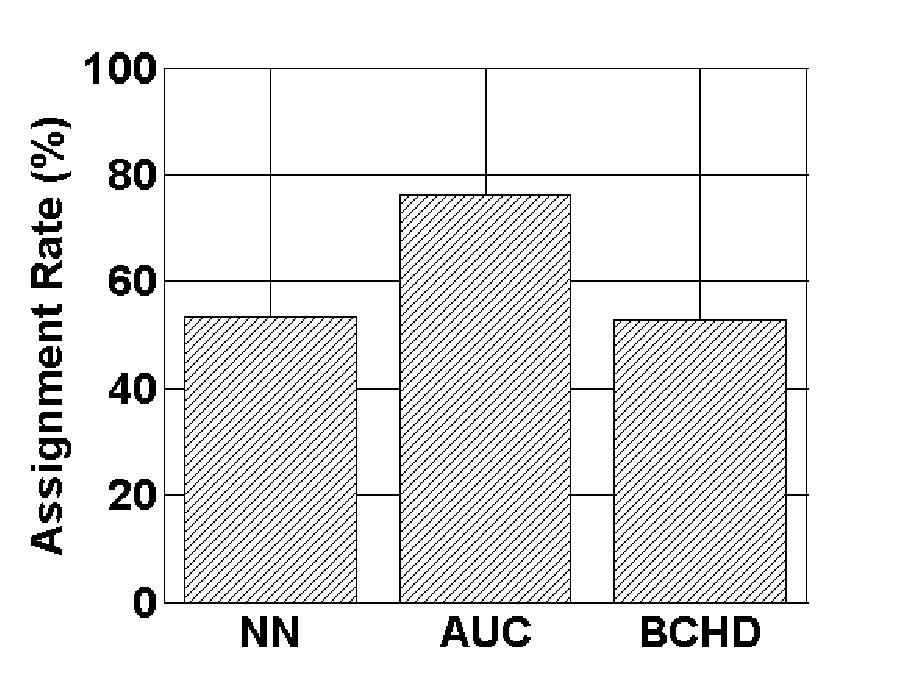
\includegraphics[width = 0.45\columnwidth]{figures/gowalla.eps}
    }
    \subfigure[Foursquare]{
        \label{fig:foursquare}
        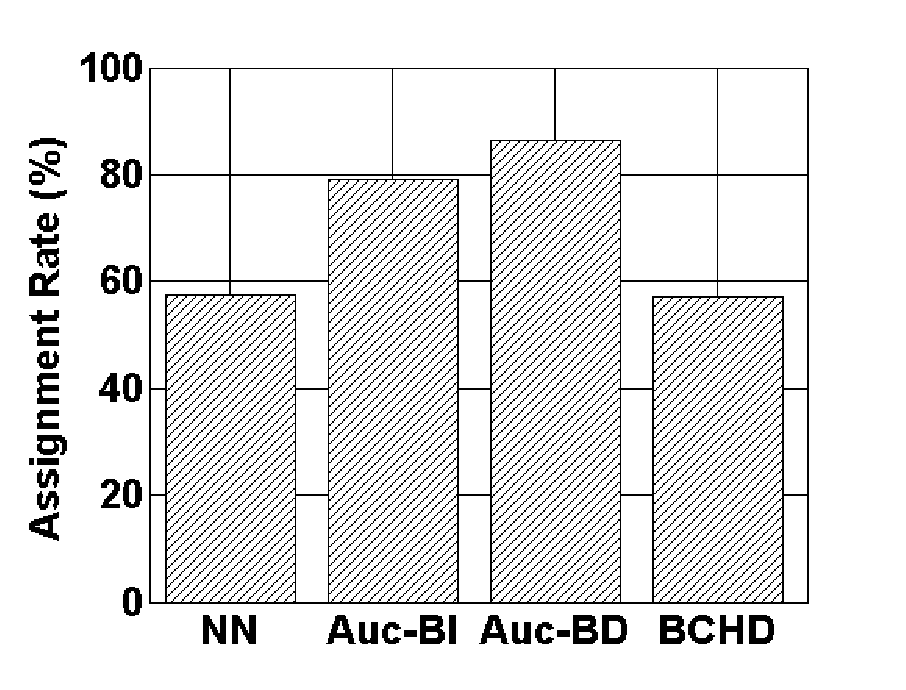
\includegraphics[width = 0.45\columnwidth]{figures/foursquare.eps}
    }
    \subfigure[Synthetic]{
        \label{fig:syn}
        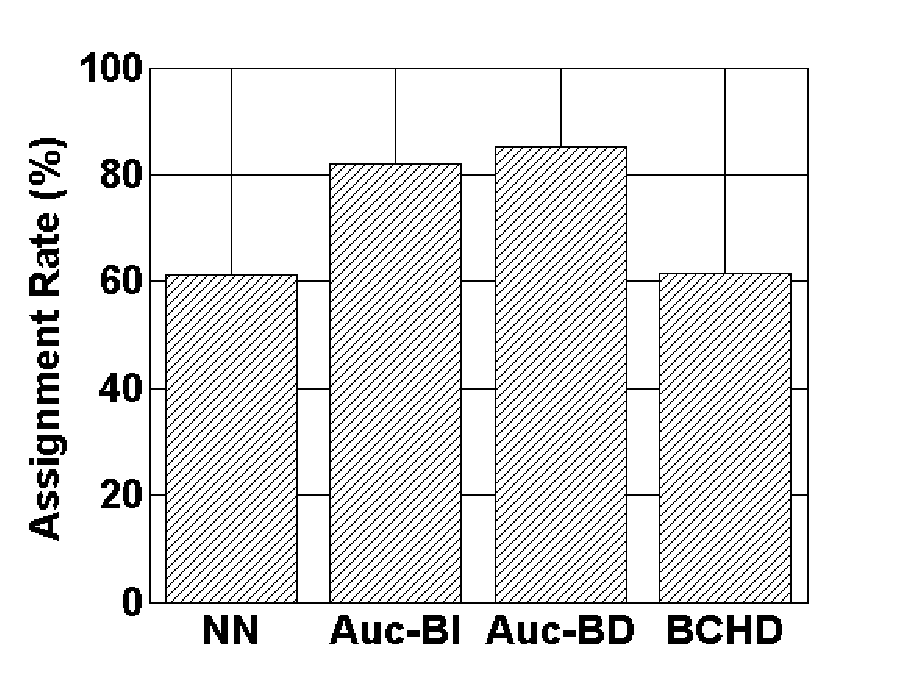
\includegraphics[width = 0.45\columnwidth]{figures/syn.eps}
    }
    \vspace{-0.15in}
    \caption{Assignment Quality of Real-Time Approaches}
    \label{fig:quality}
\end{figure}

\cref{fig:quality} compares the assignment quality of different real-time algorithms. As we can see, both SC approaches outperforms the best non-SC algorithm by almost 25\%. The main reason as explained in \cref{sec:onlinealgo} is that, the SC rules perform scheduling when matching tasks with workers. Also, BD outperforms BI by at most 10\%. This is not surprising as BD tends to ``move" workers to areas where future tasks are more likely to appear, thus achieving higher assignment in long term. Among the non-SC approaches NN outperforms other rules by almost 2 times more completed tasks. The reason MFT does not outperform RNK can be explained by what we call a \emph{radical move}. A \emph{radical move} is when the SC-Server assigns a task to a worker which requires it to move a relatively long distance to reach the location of that task. Since we do not consider any spatial proximity to the task with MFT, there is a high chance to end up with assignments resulting in radical moves. With NN and BI the general idea is to prevent radical moves as much as possible. With BD, although radical moves occur, but only if the worker moves to areas where there will be more tasks to complete.\\

Furthermore, SC bidding rules (i.e.; BI and BD) outperform BCHD by almost a similar margin. One reason is that BCHD performs the matching phase and then attempts to schedule tasks for their matched workers. All tasks that could not be scheduled for their matched workers, will go back to the matching phase and the process continues until all tasks are scheduled or there is no more worker to match with a task. When performing the matching, the schedule of the worker is not considered and hence a task might end up getting matched to and scheduled for a worker that was not the best worker. This in turn, can lower the chances of that worker to get assigned to a new task in the future. The second reason is that while a task is waiting at the server to get processed with the next batch, depending on the length of the batching  interval, it will lose some portion of its available time before its deadline, which in turn, can lower the chances of the task fitting a worker's schedule (more details in \cref{subsec:exp_scale}).\\

\begin{figure}[h]
    \centering
    \subfigure[RNK]{
        \label{fig:rnk_comp}
        \includegraphics[width = 0.45\columnwidth]{figures/rnk.eps}
    }
    \subfigure[MFT]{
        \label{fig:mft_comp}
        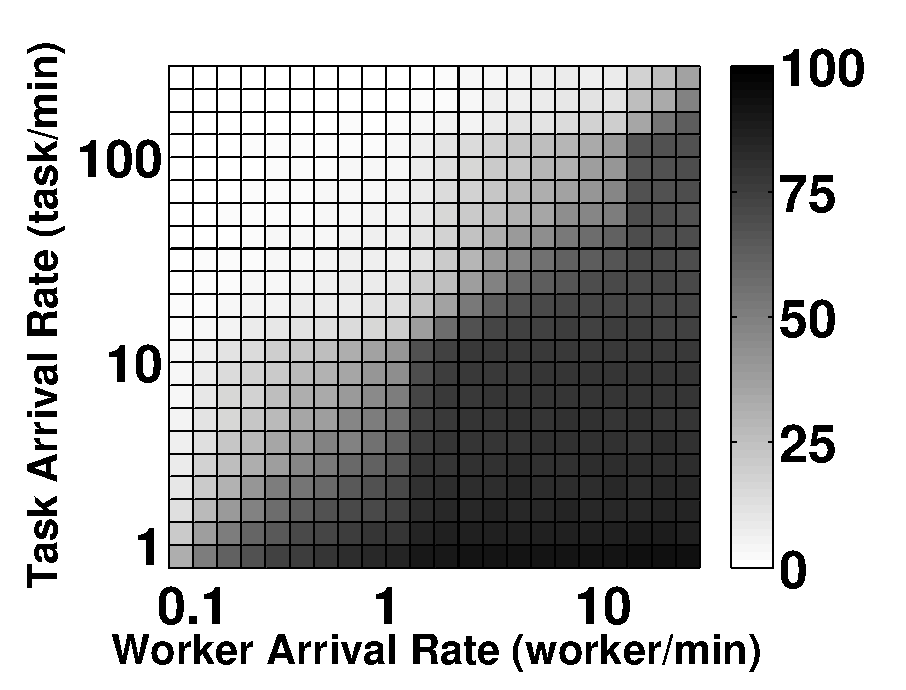
\includegraphics[width = 0.45\columnwidth]{figures/mft.eps}
    }
    \subfigure[NN]{
        \label{fig:nn_comp}
        \includegraphics[width = 0.45\columnwidth]{figures/nn.eps}
    }
    \subfigure[BI]{
        \label{fig:bi_comp}
        \includegraphics[width = 0.45\columnwidth]{figures/bi.eps}
    }
    \subfigure[BD]{
        \label{fig:emd_comp}
        \includegraphics[width = 0.45\columnwidth]{figures/emd.eps}
    }
    \subfigure[BCHD]{
        \label{fig:bchd_comp}
        \includegraphics[width = 0.45\columnwidth]{figures/bchd.eps}
    }
    \vspace{-0.15in}
    \caption{\small{Assignment Profile-Varying Worker/Task Arrival Rates}}
    \label{fig:tw_rate}
\end{figure}

In order to study the effect of temporal parameters of SC, we ran several experiments using different pairs of task arrival rates ($t_{rate}$) and worker arrival rates ($w_{rate}$). In \cref{fig:tw_rate} we show the effect of increasing $t_{rate}$ and $w_{rate}$ on the quality of the assignment. The level of grayness corresponds to the percentage of completed tasks with black and white representing 100\% and 0\%, respectively. As we can see with small number of workers, as we increase the task arrival rate, the percentage of completed tasks decreases where at the top left corner of each plot we get close to 0\%. On the other hand with small number of incoming tasks, as we increase $w_{rate}$, eventually all tasks will be completed. \cref{fig:tw_rate} shows that among non-SC rules NN outperform RNK and MFT independent of the $t_{rate}$ and $w_{rate}$ and hence, for the remainder of experiments, we only consider NN among non-SC rules.

\begin{figure}[h]
	\centering
	\includegraphics[width = 0.65\columnwidth]{figures/bi_nn.eps}
	\vspace{-0.1in}
	\caption{Assignment Difference of BI Vs. NN}\label{fig:bi_nn}
\end{figure}

\begin{figure}[h]
	\centering
	\includegraphics[width = 0.65\columnwidth]{figures/bi_bchd.eps}
	\vspace{-0.1in}
	\caption{Assignment Difference of BI Vs. BCHD}\label{fig:bi_bchd}
\end{figure}

\begin{figure}[h]
	\centering
	\includegraphics[width = 0.65\columnwidth]{figures/emd_bi.eps}
	\vspace{-0.1in}
	\caption{Assignment Difference of BD Vs. BI}\label{fig:emd_bi}
\end{figure}

To better evaluate the leading approaches, NN, BI, BD and BCHD, in \cref{fig:rate_comp} we performed a pair-wise comparison by taking their task completion rates. For example, \cref{fig:bi_nn} shows the difference between BI and NN. We observe that all approaches perform similarly at the two extreme cases discussed in \cref{fig:tw_rate}, i.e., high task-low worker and low task-high worker. BI outperform NN and BCHD up to 30\% when the problem is more complex, i.e., outside the extreme cases. An interesting observation in \cref{fig:bi_nn} is that BI outperforms NN by a larger margin at scale (higher $t_{rate}$ and $w_{rate}$). The reason is that with higher $t_{rate}$ and $w_{rate}$ more workers are moving around and more tasks come and leave so in general the spatiotemporal dynamism of the system increases. BI and BD cope with the dynamism by guaranteeing a task gets assigned to worker that can complete it. On the contrary, NN ignores the schedule of a worker during matching and this becomes more important as there is more dynamism in the system.

\begin{figure}[h]
	\centering
	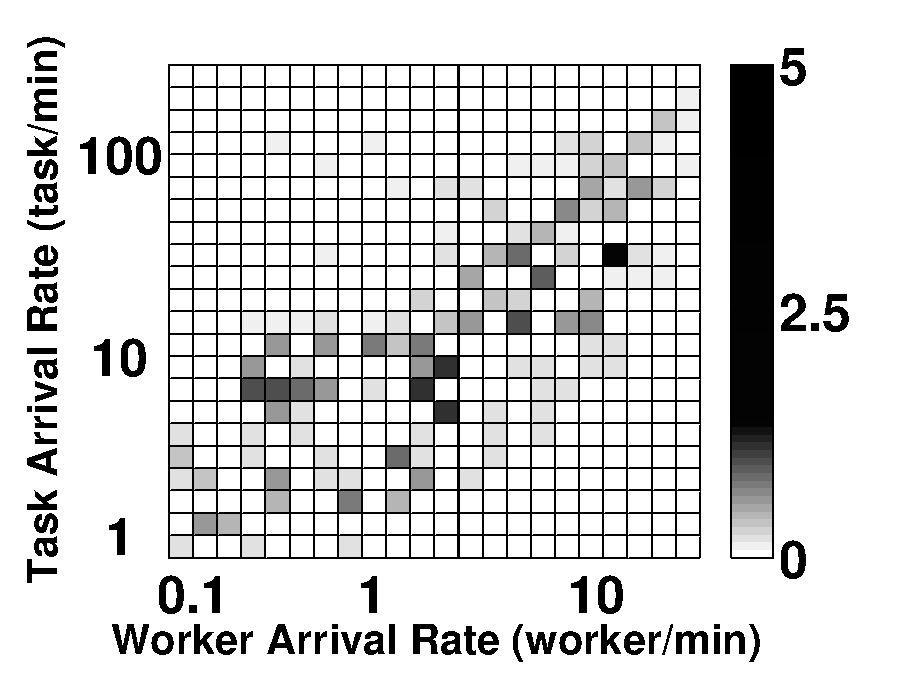
\includegraphics[width = 0.75\columnwidth]{figures/bi_abi.eps}
	\vspace{-0.1in}
	\caption{Assignment Difference of BI Vs. ApproxBI}\label{fig:bi_abi}
\end{figure}

We mentioned earlier that with the SC-rules, the workers perform an exhaustive search to find out if they can fit a new task into their schedule. As workers accept new tasks, they also complete some other tasks so as we observed in our experiments, performing an exhaustive search did not cause any scalability issues. Nevertheless, one might want to replace the exhaustive search with a polynomial time approximate algorithm. With ApproxBI, we use the insertion algorithm from \cite{Rosenkrantz74} that runs in $O(n^2)$. \cref{fig:bi_abi} shows the change affects the quality of the assignment by less than 5\%. The difference caused by ApproxBI is that the workers that are eligible for a task using BI, may not be able to fit the task in their schedules using ApproxBI due to the approximation. As a result, using ApproxBI the server may not be able to assign some tasks even if they can be completed using BI. Fortunately, as shown in \cref{fig:bi_abi}, that does not happen very often regardless of $t_{rate}$ and $w_{rate}$.

The next set of experiments compare the effect of the spatial distribution of tasks. We compared the quality of the final assignment for three different distribution. Even though real-world data usually follow a skewed spatial distribution (\cref{subsec:dataset}), the results of these experiments show that regardless of the distribution, BI and BD outperform NN and BCHD. With the first distribution, the location of the tasks follow a spatial Poisson process \cite{Baddeley07}. The other two distributions are a Uniform 2D distribution and a Skewed distribution. The results in \cref{fig:dists} show that BI and BD generate assignments at least 20\% better than NN and BCHD. Also, we can see with Poisson and Uniform distributions, there is not much difference between BI and BD. The reason is that both distributions generate tasks at completely random locations. Consequently, tasks are released at every area with the same probability and hence BD and BI become similar.

\begin{figure}[h]
	\centering
	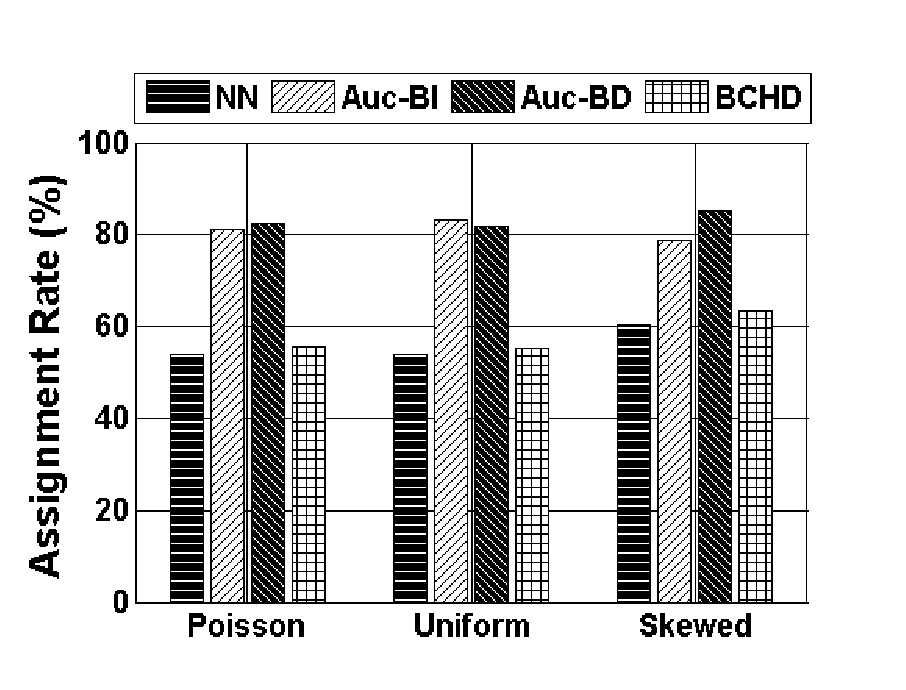
\includegraphics[width=0.75\columnwidth]{figures/dists.eps}
	\vspace{-0.1in}
	\caption{Assignment Difference-Varying Distribution}\label{fig:dists}
\end{figure}

Earlier we explained for some use cases (e.g., Uber), batched assignment does not even satisfy application requirements. Nevertheless, the results in \cref{fig:bi_lals} show even if non real-time assignments are tolerable, the quality of batched assignment is not as good as the online assignment. 


\subsection{Scalability}
\label{subsec:exp_scale}
The last set of experiments focus on measuring the scalability of BCHD, Auction-SC and a monolithic server. We compare the scalability of BI and BD bidding rules in Auction-SC (i.e., \textbf{A-BI} and \textbf{A-BD}) with the equivalent implementation of the same algorithms on a monolithic SC-Server.  and call them \textbf{M-BI} and \textbf{M-BD}.

We can measure the scalability of SC systems by their throughput: the number of tasks processed per second , or equivalently, the processing time per task, shown in \cref{fig:runtime}. Since Auction-SC utilizes the workers for scheduling an incoming task, In \cref{fig:runtime} we see that the average processing time of a single task does not change as the arrival rate of workers increases. On the contrary, with the M-BI, M-BD and BCHD, the average processing time of a single task increases linearly as we increase the number of workers and is several orders of magnitude higher than A-BI and A-BD. 

\begin{figure}[h]
    \centering
    \subfigure[M-BI]{
        \label{fig:runtime_mbi}
        \includegraphics[width = 0.45\columnwidth]{figures/run_time_mbi.eps}
    }
    \subfigure[A-BI]{
        \label{fig:runtime_abi}
        \includegraphics[width = 0.45\columnwidth]{figures/run_time_abi.eps}
    }
    \subfigure[M-BD]{
        \label{fig:runtime_mbd}
        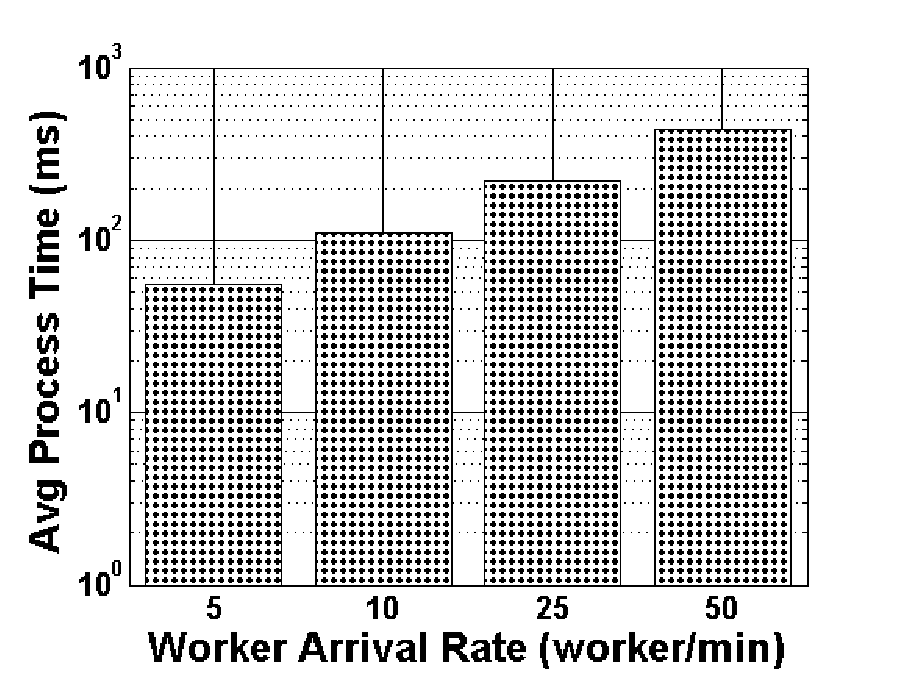
\includegraphics[width = 0.45\columnwidth]{figures/run_time_mbd.eps}
    }
    \subfigure[A-BD]{
        \label{fig:runtime_abd}
        \includegraphics[width = 0.45\columnwidth]{figures/run_time_abd.eps}
    }
    \subfigure[BCHD]{
        \label{fig:runtime_bchd}
        \includegraphics[width = 0.45\columnwidth]{figures/run_time_bchd.eps}
    }
    \vspace{-0.15in}
    \caption{Average processing time for a single task}
    \label{fig:runtime}
\end{figure}

For a \emph{CEP} engine, it is also common to measure the queuing delay of events \cite{Wu06} once they arrive at the system as a metric for the scalablility of the systems. In \cref{fig:queue} we compare the average queuing delay of tasks for A-BI, A-BD, M-BI and M-BD after running them for 1 hour (Because BCHD does not process tasks one task at a time, the concept of queuing delay is irrelevant). We can see that monolithic-SC suffers from queuing delays with less than 10 tasks/second. On the other hand, with Auction-SC, even for BD, we do not observe queuing delays for up to 50 tasks/second.

\begin{figure}[h]
	\centering
	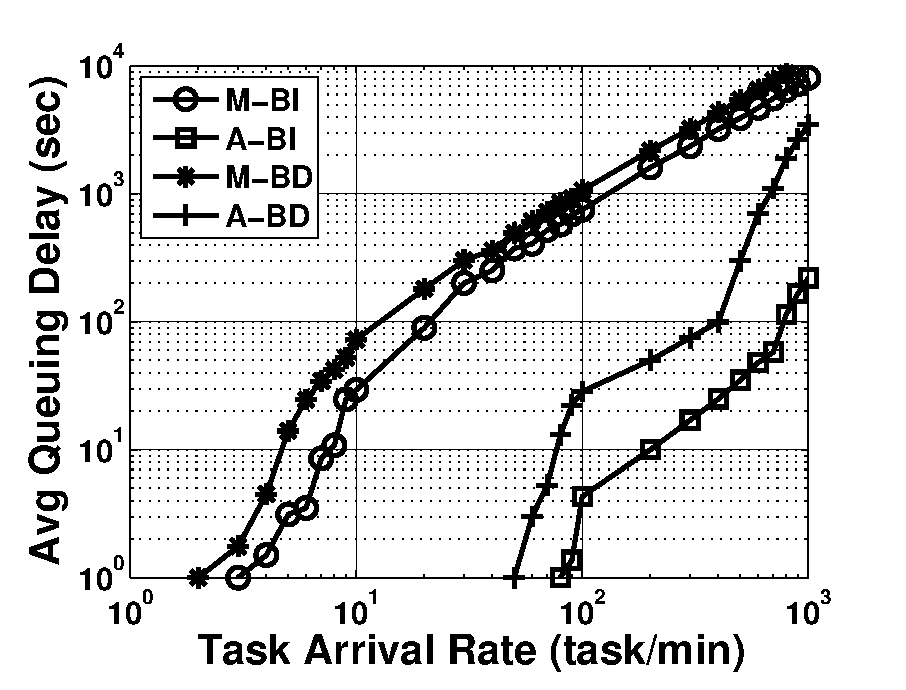
\includegraphics[width = 0.75\columnwidth]{figures/queue.eps}
	\vspace{-0.1in}
	\caption{Average queuing delay}\label{fig:queue}
\end{figure}

Earlier, we explained that with BCHD, as task has to wait in a queue for the server to finish processing an earlier batch. Depending, on the batching interval, the negative effect of batching can propagate over time. For example, if we start with a batching interval of 1 second while having a task arrival rate of 10 tasks/second, the first batch will run with \textasciitilde 10 tasks. If processing the first batch takes 2 seconds, by the time we want to process the second batch \textasciitilde 20 tasks have been queued and have to be process. Consequently, the second batch will take longer than two seconds and so on so forth. In \cref{fig:bs} we run BCHD with a task arrival rate of 10 tasks/second. We measure the following three metrics for different batches over time: (1) the number of tasks per batch, (2) the processing time of each batch and (3) the average delay of each task before its processed (i.e., the duration between the time the task arrives in the system and the time its processing starts). \cref{fig:bs} shows how the negative effects of batching propagates over time.

\begin{figure}[h]
    \centering
    \subfigure[Tasks per Batch]{
        \label{fig:bs_tpb}
        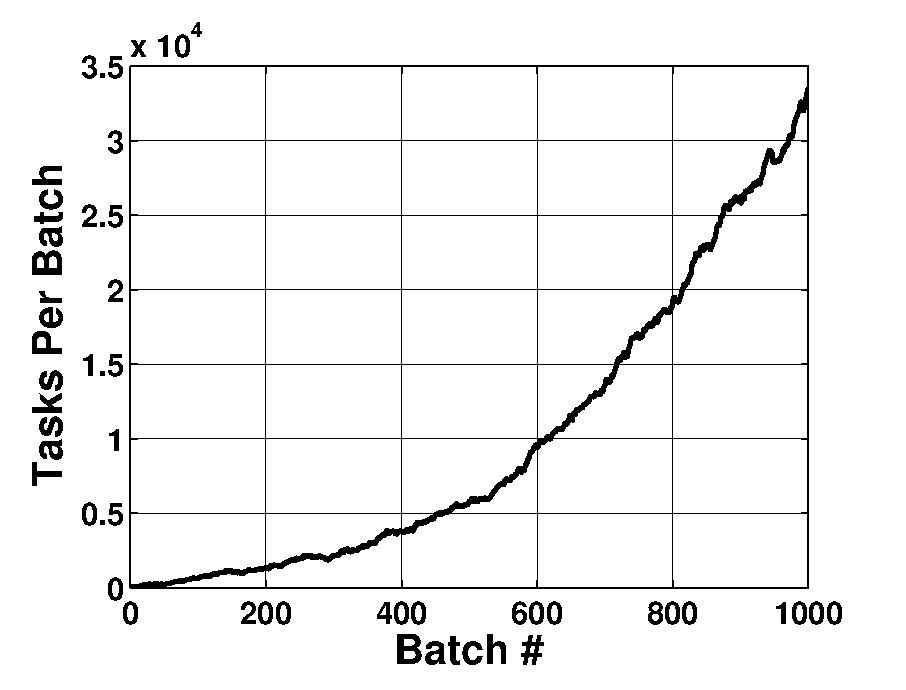
\includegraphics[width = 0.45\columnwidth]{figures/bs_tpb.eps}
    }
    \subfigure[Batch Processing Time]{
        \label{fig:bs_bpt}
        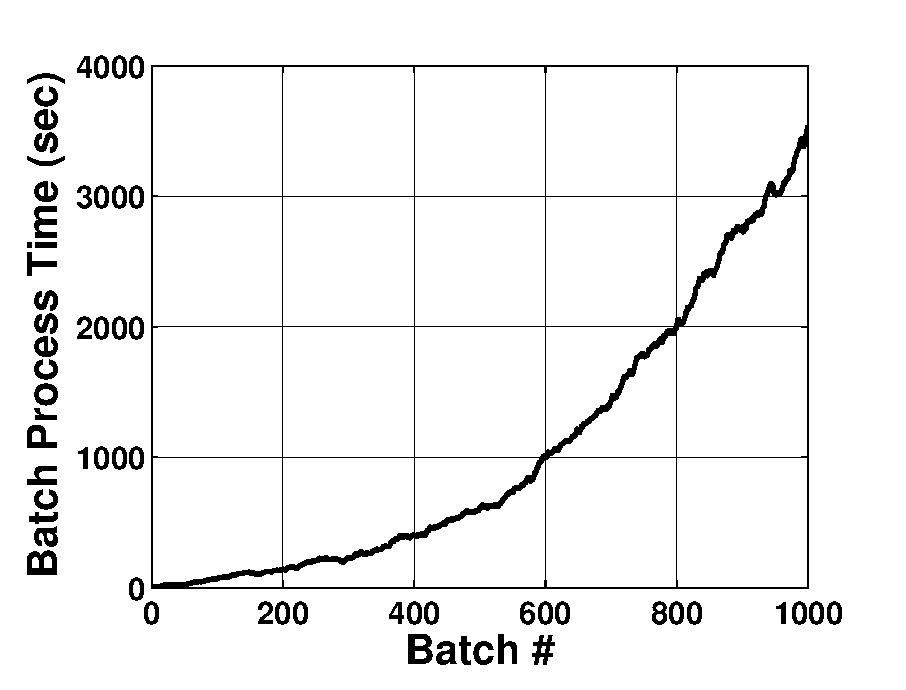
\includegraphics[width = 0.45\columnwidth]{figures/bs_bpt.eps}
    }
    \subfigure[Task Avg Delay per Batch]{
        \label{fig:bs_tad}
        \includegraphics[width = 0.45\columnwidth]{figures/bs_tad.eps}
    }
    \vspace{-0.15in}
    \caption{BCHD Scalability ($tRate = 10 task/minute$)}
    \label{fig:bs}
\end{figure}

\cref{fig:bss} shows the same three metrics when varying the task arrival rate. As it can be seen, for task arrival rates smaller then 10 tasks/second, the processing time of each batch doesn't change over time. However, for a task arrival rate of only 10 tasks/second, BCHD can no longer scale.

\begin{figure}[h]
    \centering
    \subfigure[Tasks per Batch]{
        \label{fig:bs_tpb}
        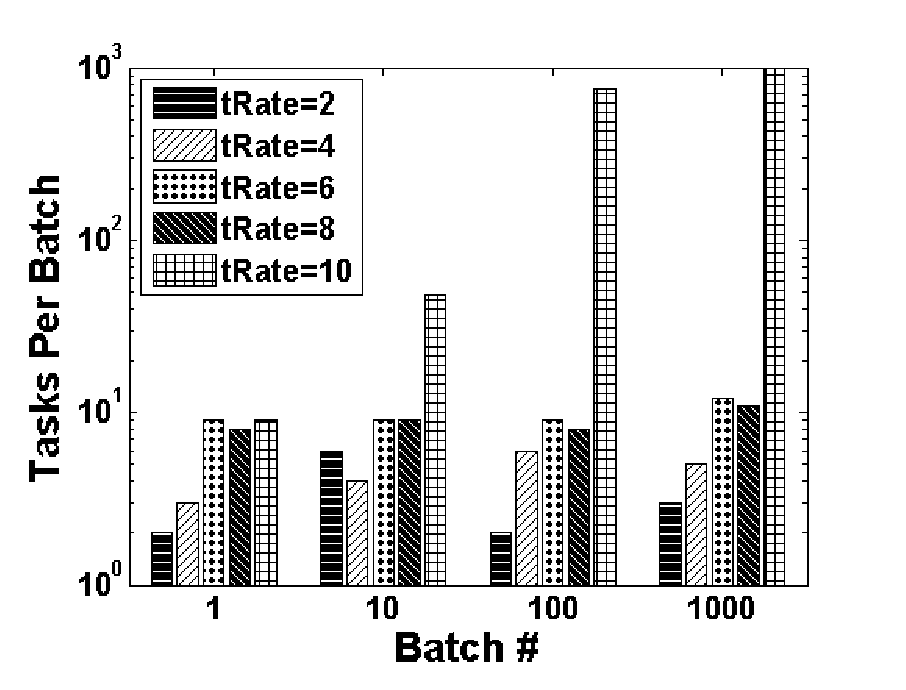
\includegraphics[width = 0.45\columnwidth]{figures/bss_tpb.eps}
    }
    \subfigure[Batch Processing Time]{
        \label{fig:bs_bpt}
        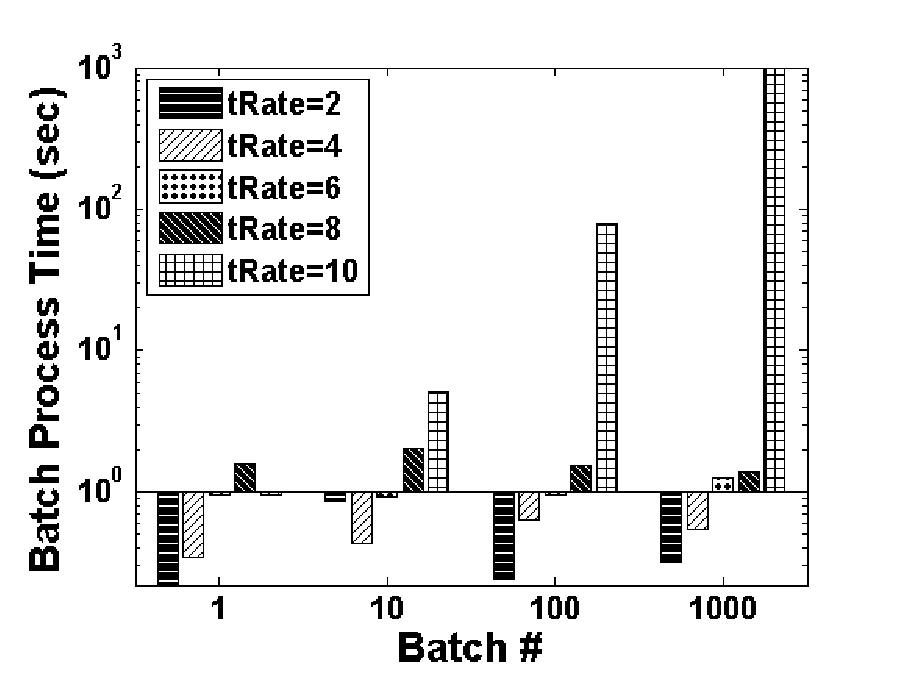
\includegraphics[width = 0.45\columnwidth]{figures/bss_bpt.eps}
    }
    \subfigure[Task Avg Delay per Batch]{
        \label{fig:bs_tad}
        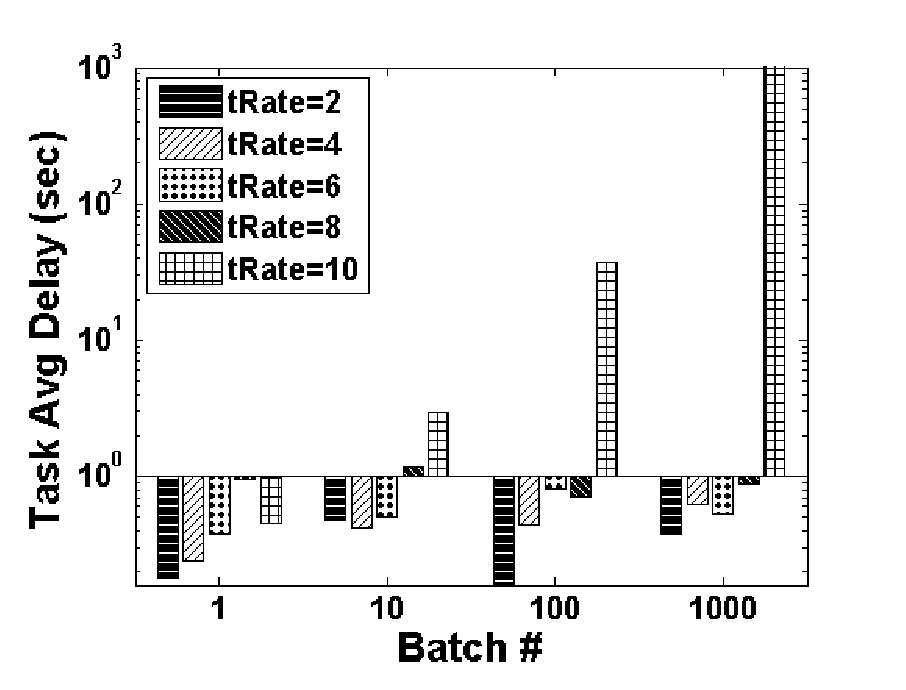
\includegraphics[width = 0.45\columnwidth]{figures/bss_tad.eps}
    }
    \vspace{-0.15in}
    \caption{BCHD Scalability}
    \label{fig:bss}
\end{figure}

To provide a more practical perspective, in \cref{fig:req} we compare the scalability of different approaches given the current requirements of a ride sharing application in New York City \cite{NYCTaxi}. As shown, while M-BD, M-BI and BCHD cannot satisfy the current requirements, Auction-SC can scale much higher than what currently is needed.

\begin{figure}[h]
	\centering
	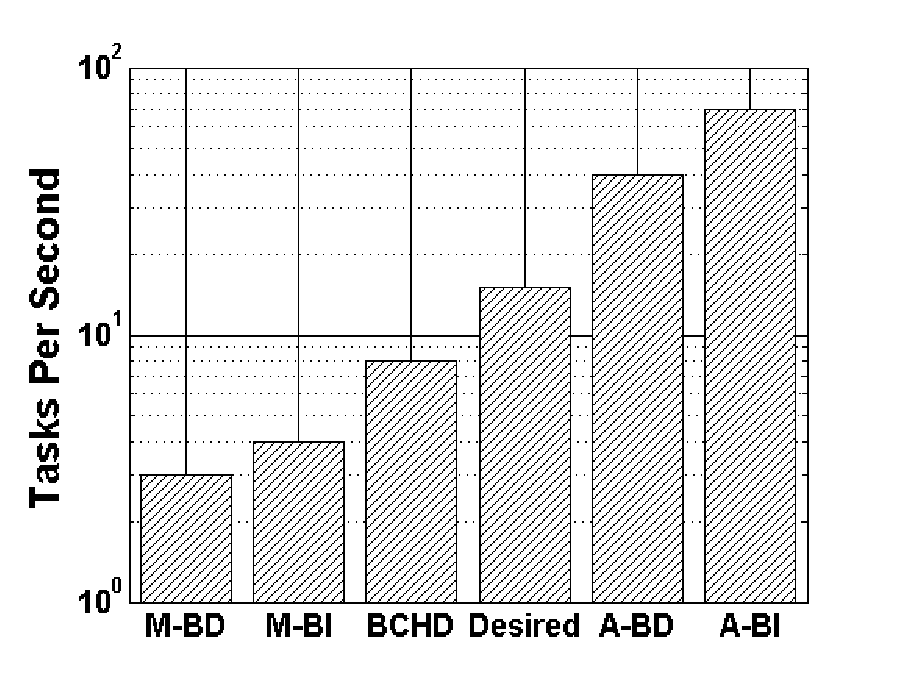
\includegraphics[width = 0.75\columnwidth]{figures/scale_req.eps}
	\vspace{-0.1in}
	\caption{Real-world Scalability Requirements}\label{fig:req}
\end{figure}

To summarize the results of our experiments, we showed that when SC bidding rules are used, the quality of the assignment is much higher as compared to when BCHD or a non-SC rule is used. The consideration of scheduling at the time a task is being matched is the main reason for the better overall assignments. When running on a monolithic SC-Server, neither one of bidding rules can scale. Furthermore, the time required to process a single task increases linearly as more workers are added to the system except for Auction-SC. On the other hand , Auction-AC can afford to execute complex SC bidding rules, resulting in a very high quality assignment. Finally, BD incurs higher delay than BI but results in higher completion rates (\cref{fig:quality,fig:emd_bi}). Users of Auction-SC can choose between BD and BI to balance their needs for assignment quality and efficiency.
%\cref{tab:summary} shows the summary of our experimental results.

%\begin{table*}
%  \centering
%  \begin{tabular}{|c|c|c|c|c|c|c|c|c|}
%    \hline
%    \multicolumn{2}{|>{\columncolor{kugray5}}c|}{}&\multicolumn{4}{c|}{non-SC bidding rules}&\multicolumn{2}{c|}{SC bidding rules}\\
%    \arrayrulecolor{kugray5}
%    \arrayrulecolor{black}
%    \cline{3-8}
%    \multicolumn{2}{|>{\columncolor{kugray5}}c|}{}&Rnd&Rnk&NN&MFT&BI&BD\\
%    \hline
%    \multirow{2}{*}{Centralized}&Scalability&Bad&Bad&Bad&Bad&Very Bad&Very Bad\\
%    \cline{2-8}
%                         		&Assignment Quality&Very Bad&Very Bad&Bad&Very Bad&Very Good&Very Good\\
%    \hline
%    \multirow{2}{*}{Auction-SC}&Scalability&Very Good&Very Good&Very Good&Very Good&Good&Good\\
%    \cline{2-8}
%                         		&Assignment Quality&Very Bad&Very Bad&Bad&Very Bad&Very Good&Very Good\\
%    \hline
%  \end{tabular}
%  \vspace{-0.1in}
%  \caption{Summary of Experimental Results}
%  \label{tab:summary}
%\end{table*}

\section{Conclusion and Future Work}
\label{sec:future}

In this paper, we studied the problem of real-time task assignment and scheduling in spatial crowdsourcing. We showed that neither of the two current approaches for task assignment in spatial crowdsourcing, batched assignment and centralized online assignment, can scale as either task matching or task scheduling will become the bottleneck. Therefore, we introduced an auction-based framework in which we split the matching and scheduling responsibilities between SC-Server and workers, respectively. We showed that by exploiting the spatiotemporal aspects of SC, with our proposed algorithms, the workers will be able to complete up to 30\% more tasks as compared to non-SC approaches. The decentralized architecture of our framework allows for performing such high quality assignments at scale.

In this paper, we assumed each task can be performed instantaneously, e.g., taking a picture. Once that assumption is relaxed, we will face new challenges with scheduling the tasks. We also assumed each task requires the worker to travel to a single location. However, in other applications the worker may need to visit multiple locations for a single task, e.g., in the Uber application the worker has to pick up a passenger at one location and drop him off at a second location. We plan to extend our Auction-SC framework to incorporate these two features.

\begin{scriptsize}
\bibliographystyle{IEEEtran}
\bibliography{spatialcrowdsourcing}
\end{scriptsize}

%\appendix

\begin{appendices}

\section{Proof of Theorem 1}
\label{app:MinHamProof}
In order to prove NP-Hardness of Min-Ham-Path we show Ham-Path $\leq_p$ Min-Ham-Path. The Hamiltonian Path problem asks the following question: Given a directed graph $G(V,E)$ does there exist a path that goes through every node exactly once?\\

Given and instance of the Ham-Path problem $\left\langle G \right\rangle$ we modify graph $G(V,E)$ and generate a new graph $G'(V', E')$ where $V' = V \cup \left\{ o \right\}$ and $E' = E \cup \left\{ \left\langle o, v \right\rangle : v \in V \right\}$. Also, for every $e \in E'$ we Assume $l(e) = 1$.\\

Now we show that Ham-Path$\left\langle G \right\rangle$ is true \emph{iff} Min-Ham-Path$\left\langle G', l, o, n \right\rangle$ is true where $n$ is the number of vertices in $G$. If Min-Ham-Path returns a path of length $n$, we can remove the first edge from the path which will result in a Hamiltonian Path for the Ham-Path$\left\langle G \right\rangle$ problem. On the other hand every Hamiltonian Path on graph $G$ will have length $n-1$. By adding vertex $o$ and connecting it to the starting vertex, we end up with a Hamiltonian Path of length $n$ on $G'$.

\section{Proof of Theorem 2}
\label{app:TASCProof}
We start the proof by showing that the decision problem of TASC is NP. Given a matching M, we can check that no task is assigned to more than one worker in polynomial time. Also, we can find the value of M with a adding the value of every task in M.\\

Now we prove TASC is NP-Hard by Min-Ham-Path $\leq_p$ TASC. Given an instance of the Min-Ham-Path problem $\left\langle G(V,E), l, o, K \right\rangle$ we reduce it to an instance of the TASC$\left\langle W, T, l', n \right\rangle$ problem such that $W = \left\{ o \right\}$, $T = V \setminus \left\{ o \right\}$. For every task $t$ we set $t.v = 1$, $t.r = 0$ and $t.d = K$ (We assume workers travel one unit of length with every unit of time). Also for every $e \in E, l'(e) = l(e)$. In addition for every $e' \in \left( W \times T \right) \cup \left( T \times T \right) $ where $e' \not\in E$ we set $l'(e') = \infty$.\\ 

Finally we show the result of Min-Ham-Path$\left\langle G, l, o, K \right\rangle$ is true if TASC$\left\langle W, T, l', n-1 \right\rangle$ is true where $n$ is the number of vertices in $G$. Considering that $\left\vert T \right\vert = n - 1$ and $t.v = 1$ for every $t \in T$, if there exists a matching with size $n - 1$ it means every task has been assigned to the single worker. Also, since we set the deadline of every task to $K$ this means the worker visits every task no later than $K$. Therefore, the path that the worker traverses starts at $o$ and goes through every other vertex $v \in V \setminus \left\{ o \right\}$ where the length of the path is no more than $K$.

\end{appendices}

\end{document}